\documentclass[12pt]{article}
\usepackage[a4paper, inner=1.5cm, outer=3cm, top=2cm,bottom=3cm, bindingoffset=1cm]{geometry}
\usepackage[english]{babel}
\usepackage[utf8x]{inputenc}
\usepackage[nottoc]{tocbibind}
\usepackage{import}
\usepackage{nomencl}
\usepackage{amsmath}
\usepackage{tikz}
\usepackage[maxfloats=256]{morefloats}
\usepackage{booktabs}
\usepackage{graphicx}
\usepackage{hyperref}
\usepackage{pdflscape}
\usepackage{adjustbox}
\graphicspath{ {./images/} }
\usepackage{capt-of} 
\usepackage{listings}
\usepackage{xcolor}
\usepackage{multirow}
\usepackage{setspace}
\definecolor{codegreen}{rgb}{0,0.6,0}
\definecolor{codegray}{rgb}{0.5,0.5,0.5}
\definecolor{codepurple}{rgb}{0.58,0,0.82}
\definecolor{backcolour}{rgb}{0.95,0.95,0.92}

\maxdeadcycles=1000

\lstdefinestyle{mystyle}{
    backgroundcolor=\color{backcolour},   
    commentstyle=\color{codegreen},
    keywordstyle=\color{magenta},
    numberstyle=\tiny\color{codegray},
    stringstyle=\color{codepurple},
    basicstyle=\ttfamily\footnotesize,
    breakatwhitespace=false,         
    breaklines=true,                 
    captionpos=b,                    
    keepspaces=true,                 
    numbers=left,                    
    numbersep=5pt,                  
    showspaces=false,                
    showstringspaces=false,
    showtabs=false,                  
    tabsize=2
}
 
\lstset{style=mystyle}

\begin{document}
\begin{titlepage}
\newcommand{\HRule}{\rule{\linewidth}{0.5mm}} 
\center
\doublespacing
\textbf{\Huge MACHINE LEARNING FOR PREDICTING DIABETES MELLITUS}
\\
\singlespacing
\Large
\vspace{3cm}
A project report submitted in partial fulfilment of the requirement for the degree of\\
\vspace{1cm}
\textbf{Bachelor in Science\\In\\Computer Science}
\\by\\
\Large
Alexander Roque Rodrigues
\\
\vspace{1cm}
under the supervision of
\vspace{1cm}
\\
Ashweta Fondekar
\\
\vspace{3cm}
\textbf{PARVATIBAI CHOWGULE COLLEGE OF ARTS \& SCIENCE AUTONOMOUS}
\\June 2019
\end{titlepage}

%declaration
\onehalfspacing
%\doublespacing
\newpage
\vspace{15cm}
\begin{center}

\Huge{\textbf{Declaration by Candidate}}\\
\normalsize
I declare that this project report has been prepared by me and to the best of my
knowledge, it has not previously formed the basis for the award of any diploma or degree by
any other University.
\end{center}
\newpage
\vspace{15cm}

\begin{center}
\Huge{\textbf{Certificate by Supervisor}}\\
\normalsize
Certified that the Project Report is a record of work done by the candidate himself/herself/themselves under my guidance during the period of study and that to the best of my knowledge, it has not previously formed the basis of the award of any degree or diploma of any other University.\\
\vspace{5cm}
Ashweta Fondekar\\

Project Supervisor
\end{center}
\newpage

\textbf{Work Record}


\newpage
\section{Acknowledgements}

\newpage
\tableofcontents
\newpage
\listoffigures
\newpage
\listoftables
\newpage
\makenomenclature
\newpage


\begin{abstract}
Diabetes Mellitus is a disease that prevents the body from properly expanding the
energy stored from the food consumed. The purpose of this project was to select
machine learning algorithms that are able to predict or classify a person as diabetic
or healthy based on the legacy data. The algorithms compared were KNN
Classifier, Logistic Regression, Decision Tree Classifier, Random Forest
Classifier, Gradient Boosting Classifier, Support Vector Classifier and the
Multi-Layered Perceptron. From all the above the Multi-Layered Perceptron gave
an accuracy of prediction on the dataset as ~79.70\%. To improve the performance
of the classifier, I have considered new features deduced from the currently
existing feature set a re-trained the classifier on the new dataset that I generated,
which is now able to classify the subject as diabetic or healthy with a new accuracy
of ~85.42\%. After selection of the algorithm I further advanced the platform of cluster computing to
deploy the algorithm onto and generate predictions in without any human
interference​ and also made the data available
to the users via an easy to use web application which gives them access to the
observations then stored in the database after being predicted by the algorithm
deployed on the nodes.
\end{abstract}


\section{Introduction}
In recent days, there has been a sharp increase in the cases of diabetes mellitus. Diabetes mellitus is on the rise amongst many people and the rate of contracting this lifestyle disease could be reduced significantly if proper measures and precautions were to be instilled amongst people the number of people can be reduced.

Machine learning is a growing field in computer science. With the development and introduction of many algorithms the prediction and accuracy of the predictions itself has improved substantially. Machine learning and healthcare systems are also becoming increasingly popular in the healthcare sector.

The project encompasses the qualities of Remote Patient Monitoring (RPM) and Clinical Decision Support (CDS). RPM provides medical facilities that have the ability to transmit patient data to healthcare professionals who might very well be halfway around the world. RPM can monitor blood glucose levels and blood pressure. It is particularly helpful for patients with chronic conditions such as type 2 diabetes, hypertension, or cardiac disease. Data collected and transmitted via PRM can be used by a healthcare professional or a healthcare team to detect medical events such as stroke or heart attack that require immediate and aggressive medical intervention. Data collected may be used as part of a research project or health study. RPM is a life-saving system for patients in remote areas who cannot access face-to-face health care. CDS analyzes data from clinical and administrative systems. The aim is to assist healthcare providers in making informed clinical decisions. Data available can provide information to medical professions who are preparing diagnoses or predicting medical conditions like drug interactions and reactions. CDS tools filter information to assist healthcare professionals in caring for individual clients. 

Cluster computing or High-Performance computing frameworks is a form of computing in which bunch of computers (often called nodes) that are connected through a LAN (local area network) so that, they behave like a single machine. A computer cluster help to solve complex operations more efficiently with much faster processing speed, better data integrity than a single computer and they only used for mission-critical applications.

The objective of this project is to create a  system that is able to use the machine learning algorithms and predict the outcome of the parameters entered into the algorithm and help the patient draw a conclusion whether or not he/she has the same traits exhibited by similar patients that have diabetes. Also the system should have a UI that is capable of displaying the data of the patients to the doctor and to the patients themselves for further interpretation.

\newpage
\section{Objective}
The obective of this project is to select an algorithm that is capable of classifying a healthy person from a diabetic person.

\newpage
\section{Project Rationale}

Diabetes is a chronic disease that occurs either when the pancreas does not produce enough insulin or when the body cannot effectively use the insulin it produces. Insulin is a hormone that regulates blood sugar. Hyperglycaemia, or raised blood sugar, is a common effect of uncontrolled diabetes and over time leads to serious damage to many of the body's systems, especially the nerves and blood vessels.

Taking a look at the number of people with diabetes, the count has risen from 108 million in 1980 to 422 million in 2014.
The global prevalence of diabetes among adults over 18 years of age has risen from 4.7\% in 1980 to 8.5\% in 2014. Diabetes prevalence has been rising more rapidly in middle-income and low-income countries.
Diabetes as a disease is a major cause of blindness, kidney failure, heart attacks, stroke and lower limb amputation amongst those who recognise the fatal disease late in life.
In 2016, an estimated 1.6 million deaths were directly caused by diabetes. Another 2.2 million deaths were attributable to high blood glucose in 2012. Almost half of all deaths attributable to high blood glucose occur before the age of 70 years. WHO estimates that diabetes was the seventh leading cause of death in 2016. A healthy diet, regular physical activity, maintaining a normal body weight and avoiding tobacco use are ways to prevent or delay the onset of type 2 diabetes. Diabetes can be treated and its consequences avoided or delayed with diet, physical activity, medication and regular screening and treatment for complications. In 2014, 8.5\% of adults aged 18 years and older had diabetes. In 2016, diabetes was the direct cause of 1.6 million deaths and in 2012 high blood glucose was the cause of another 2.2 million deaths.

Diabetes patients are segregated into types. Type 1 diabetes is characterized by deficient insulin production and requires daily administration of insulin. The cause of type 1 diabetes is not known and it is not preventable with current knowledge. A person with type 1 diabetes may have symptoms like excessive excretion of urine, thirst, constant hunger, weight loss, vision changes, and fatigue. These symptoms may occur suddenly.

Type 2 diabetes results from the body’s ineffective use of insulin. Type 2 diabetes comprises the majority of people with diabetes around the world, and is largely the result of excess body weight and physical inactivity. Symptoms may be similar to those of type 1 diabetes, but are often less marked. As a result, the disease may be diagnosed several years after onset, once complications have already arisen.

Until recently, this type of diabetes was seen only in adults but it is now also occurring increasingly frequently in children.

Gestational diabetes is another type of diabtetes where hyperglycaemia with blood glucose values above normal but below those diagnostic of diabetes, occurring during pregnancy. Women with gestational diabetes are at an increased risk of complications during pregnancy and at delivery. They and their children are also at increased risk of type 2 diabetes in the future. Gestational diabetes is diagnosed through prenatal screening, rather than through reported symptoms.

Untreated diabetes can damage the heart, blood vessels, eyes, kidneys, and nerves. Adults with diabetes have a two- to three-fold increased risk of heart attacks and strokes. Combined with reduced blood flow, neuropathy (nerve damage) in the feet increases the chance of foot ulcers, infection and eventual need for limb amputation. Diabetic retinopathy is an important cause of blindness, and occurs as a result of long-term accumulated damage to the small blood vessels in the retina. 2.6\% of global blindness can be attributed to diabetes. Diabetes is among the leading causes of kidney failure.

Early diagnosis can be accomplished through relatively inexpensive testing of blood sugar. Treatment of diabetes involves diet and physical activity along with lowering blood glucose and the levels of other known risk factors that damage blood vessels. Tobacco use cessation is also important to avoid complications. 

\newpage
\section{Review of Literature}
For the study I have chosen to perform a comparitive study between the K Nearest Neighbours algorithm, Logistic Regression, Decision Tree Classifier, Random Forest Classifier, Gradient Boosting Classifier, Support Vector Machine and finally a Multi Layered Perceptron for the classifier groups. 

% =============== KNN ======================

K Nearest Neighbours, is a supervised machine learning algorithm and relies on labeled input data to learn a function that produces an appropriate output when given new unlabeled data. Supervised machine learning algorithms are used to solve classification or regression problems. A classification problem has a discrete value as its output. Unlike supervised learning that tries to learn a function that will allow us to make predictions given some new unlabeled data, unsupervised learning tries to learn the basic structure of the data to give us more insight into the data. The KNN algorithm assumes that similar things exist in close proximity. In other words, similar things are near to each other. The advantages of the KNN algorithm include the reasons that the algorithm is simple and easy to implement, no need to build a model, tune several parameters, or make additional assumptions and furthermore can be used for classification, regression, and search due to its versatile nature. KNN’s main disadvantage of becoming significantly slower as the volume of data increases makes it an impractical choice in environments where predictions need to be made rapidly. Moreover, there are faster algorithms that can produce more accurate classification and regression results.
However, provided you have sufficient computing resources to speedily handle the data you are using to make predictions, KNN can still be useful in solving problems that have solutions that depend on identifying similar objects. An example of this is using the KNN algorithm in recommender systems, an application of KNN-search.

% =================== LOG REGRESSION ===================

The linear regression model can work well for regression, but fails for classification. Why is that? In case of two classes, you could label one of the classes with 0 and the other with 1 and use linear regression. Technically it works and most linear model programs will spit out weights for you. But there are a few problems with this approach:

A linear model does not output probabilities, but it treats the classes as numbers (0 and 1) and fits the best hyperplane (for a single feature, it is a line) that minimizes the distances between the points and the hyperplane. So it simply interpolates between the points, and you cannot interpret it as probabilities. A linear model also extrapolates and gives you values below zero and above one. This is a good sign that there might be a smarter approach to classification. Since the predicted outcome is not a probability, but a linear interpolation between points, there is no meaningful threshold at which you can distinguish one class from the other. 

The logistic regression algorithm even if called regression, is a classification method which is based on the probability for
a sample to belong to a class. As our probabilities must be continuous in R and bounded between (0, 1), it's necessary to introduce a threshold function to filter the term z. The name logistic comes from the decision to use the sigmoid (or logistic) function:
$$\sigma(z) = \dfrac{1}{1+e^z}$$

% =============== DECISION TREE ================

Not all problems can be solved with linear methods. The world is non-linear. It has been observed that tree based models have been able to map non-linearity effectively. Methods like decision trees, random forest, gradient boosting are being popularly used in all kinds of data science problems.

Decision Tree algorithm belongs to the family of supervised learning algorithms. Unlike other supervised learning algorithms, decision tree algorithm can be used for solving regression and classification problems too. The general motive of using Decision Tree is to create a training model which can use to predict class or value of target variables by learning decision rules inferred from prior data (training data). The primary challenge in the decision tree implementation is to identify which attributes do we need to consider as the root node and each level. Decision tress often mimic the human level thinking so it’s simple to understand the data and make some good interpretations.
Dividing efficiently based on maximum information gain is key to decision tree classifier. However, in real world with millions of data dividing into pure class in practically not feasible (it may take longer training time) and so we stop at points in nodes of tree when fulfilled with certain parameters (for example impurity percentage). Decision tree is classification strategy as opposed to the algorithm for classification. It takes top down approach and uses divide and conquer method to arrive at decision. We can have multiple leaf classes with this approach.

A decision tree is a decision support tool that uses a tree-like graph or model of decisions and their possible consequences, including chance event outcomes, resource costs, and utility. It is one way to display an algorithm that only contains conditional control statements.
A decision tree is a flowchart-like structure in which each internal node represents a “test” on an attribute (e.g. whether a coin flip comes up heads or tails), each branch represents the outcome of the test, and each leaf node represents a class label (decision taken after computing all attributes). The paths from root to leaf represent classification rules.
Tree based learning algorithms are considered to be one of the best and mostly used supervised learning methods. Tree based methods empower predictive models with high accuracy, stability and ease of interpretation. Unlike linear models, they map non-linear relationships quite well. They are adaptable at solving any kind of problem at hand (classification or regression). Decision Tree algorithms are referred to as CART (Classification and Regression Trees).

Decision trees have a natural “if … then … else …” construction that makes it fit easily into a programmatic structure. They also are well suited to categorization problems where attributes or features are systematically checked to determine a final category. For example, a decision tree could be used effectively to determine the species of an animal.

As a result, the decision making tree is one of the more popular classification algorithms being used in Data Mining and Machine Learning. Example applications include:
· Evaluation of brand expansion opportunities for a business using historical sales data
· Determination of likely buyers of a product using demographic data to enable targeting of limited advertisement budget
· Prediction of likelihood of default for applicant borrowers using predictive models generated from historical data
· Help with prioritization of emergency room patient treatment using a predictive model based on factors such as age, blood pressure, gender, location and severity of pain, and other measurements
· Decision trees are commonly used in operations research, specifically in decision analysis, to help identify a strategy most likely to reach a goal.
Because of their simplicity, tree diagrams have been used in a broad range of industries and disciplines including civil planning, energy, financial, engineering, healthcare, pharmaceutical, education, law, and business.

Decision tree is a type of supervised learning algorithm (having a pre-defined target variable) that is mostly used in classification problems. It works for both categorical and continuous input and output variables. In this technique, we split the population or sample into two or more homogeneous sets (or sub-populations) based on most significant splitter / differentiator in input variables.

Advantages of Decision Tree:
Easy to Understand: Decision tree output is very easy to understand even for people from non-analytical background. It does not require any statistical knowledge to read and interpret them. Its graphical representation is very intuitive and users can easily relate their hypothesis.
Useful in Data exploration: Decision tree is one of the fastest way to identify most significant variables and relation between two or more variables. With the help of decision trees, we can create new variables / features that has better power to predict target variable. It can also be used in data exploration stage. For e.g., we are working on a problem where we have information available in hundreds of variables, there decision tree will help to identify most significant variable.
Decision trees implicitly perform variable screening or feature selection.
Decision trees require relatively little effort from users for data preparation.
Less data cleaning required: It requires less data cleaning compared to some other modeling techniques. It is not influenced by outliers and missing values to a fair degree.
Data type is not a constraint: It can handle both numerical and categorical variables. Can also handle multi-output problems.
Non-Parametric Method: Decision tree is considered to be a non-parametric method. This means that decision trees have no assumptions about the space distribution and the classifier structure.
Non-linear relationships between parameters do not affect tree performance.
The number of hyper-parameters to be tuned is almost null.

Disadvantages of Decision Tree:
Over fitting: Decision-tree learners can create over-complex trees that do not generalize the data well. This is called overfitting. Over fitting is one of the most practical difficulty for decision tree models. This problem gets solved by setting constraints on model parameters and pruning.
Not fit for continuous variables: While working with continuous numerical variables, decision tree loses information, when it categorizes variables in different categories.
Decision trees can be unstable because small variations in the data might result in a completely different tree being generated. This is called variance, which needs to be lowered by methods like bagging and boosting.
Greedy algorithms cannot guarantee to return the globally optimal decision tree. This can be mitigated by training multiple trees, where the features and samples are randomly sampled with replacement.
Decision tree learners create biased trees if some classes dominate. It is therefore recommended to balance the data set prior to fitting with the decision tree.
Information gain in a decision tree with categorical variables gives a biased response for attributes with greater no. of categories.
Generally, it gives low prediction accuracy for a dataset as compared to other machine learning algorithms.
Calculations can become complex when there are many class label.

% ================= RANDOM FOREST ================

The random forest is a model made up of many decision trees. Rather than just simply averaging the prediction of trees (which we could call a “forest”), this model uses two key concepts that gives it the name random:
Random sampling of training data points when building trees
Random subsets of features considered when splitting nodes

When training, each tree in a random forest learns from a random sample of the data points. The samples are drawn with replacement, known as bootstrapping, which means that some samples will be used multiple times in a single tree. The idea is that by training each tree on different samples, although each tree might have high variance with respect to a particular set of the training data, overall, the entire forest will have lower variance but not at the cost of increasing the bias.
At test time, predictions are made by averaging the predictions of each decision tree. This procedure of training each individual learner on different bootstrapped subsets of the data and then averaging the predictions is known as bagging, short for bootstrap aggregating.

The random forest combines hundreds or thousands of decision trees, trains each one on a slightly different set of the observations, splitting nodes in each tree considering a limited number of the features. The final predictions of the random forest are made by averaging the predictions of each individual tree.

Decision tree: an intuitive model that makes decisions based on a sequence of questions asked about feature values. Has low bias and high variance leading to overfitting the training data.
Gini Impurity: a measure that the decision tree tries to minimize when splitting each node. Represents the probability that a randomly selected sample from a node will be incorrectly classified according to the distribution of samples in the node.
Bootstrapping: sampling random sets of observations with replacement.
Random subsets of features: selecting a random set of the features when considering splits for each node in a decision tree.
Random Forest: ensemble model made of many decision trees using bootstrapping, random subsets of features, and average voting to make predictions. This is an example of a bagging ensemble.
Bias-variance tradeoff: a core issue in machine learning describing the balance between a model with high flexibility (high variance) that learns the training data very well at the cost of not being able to generalize to new data , and an inflexible model (high bias) that cannot learn the training data. A random forest reduces the variance of a single decision tree leading to better predictions on new data.

% ============ GRADIENT BOOSTING ================

Boosting is a method of converting weak learners into strong learners. In boosting, each new tree is a fit on a modified version of the original data set. The gradient boosting algorithm (gbm) can be most easily explained by first introducing the AdaBoost Algorithm.The AdaBoost Algorithm begins by training a decision tree in which each observation is assigned an equal weight. After evaluating the first tree, we increase the weights of those observations that are difficult to classify and lower the weights for those that are easy to classify. The second tree is therefore grown on this weighted data. Here, the idea is to improve upon the predictions of the first tree. Our new model is therefore Tree 1 + Tree 2. We then compute the classification error from this new 2-tree ensemble model and grow a third tree to predict the revised residuals. We repeat this process for a specified number of iterations. Subsequent trees help us to classify observations that are not well classified by the previous trees. Predictions of the final ensemble model is therefore the weighted sum of the predictions made by the previous tree models.
Gradient Boosting trains many models in a gradual, additive and sequential manner. The major difference between AdaBoost and Gradient Boosting Algorithm is how the two algorithms identify the shortcomings of weak learners (eg. decision trees). While the AdaBoost model identifies the shortcomings by using high weight data points, gradient boosting performs the same by using gradients in the loss function (y=ax+b+e , e needs a special mention as it is the error term). The loss function is a measure indicating how good are model’s coefficients are at fitting the underlying data. A logical understanding of loss function would depend on what we are trying to optimise. For example, if we are trying to predict the sales prices by using a regression, then the loss function would be based off the error between true and predicted house prices. Similarly, if our goal is to classify credit defaults, then the loss function would be a measure of how good our predictive model is at classifying bad loans. One of the biggest motivations of using gradient boosting is that it allows one to optimise a user specified cost function, instead of a loss function that usually offers less control and does not essentially correspond with real world applications.

Hyperparameter tuning is especially significant for gbm modelling since they are prone to overfitting. The special process of tuning the number of iterations for an algorithm such as gbm and random forest is called “Early Stopping”. Early Stopping performs model optimisation by monitoring the model’s performance on a separate test data set and stopping the training procedure once the performance on the test data stops improving beyond a certain number of iterations.
It avoids overfitting by attempting to automatically select the inflection point where performance on the test dataset starts to decrease while performance on the training dataset continues to improve as the model starts to overfit. In the context of gbm, early stopping can be based either on an out of bag sample set (“OOB”) or cross- validation (“cv”). Like mentioned above, the ideal time to stop training the model is when the validation error has decreased and started to stabilise before it starts increasing due to overfitting.

How Gradient Boosting Works
Gradient boosting involves three elements:

A loss function to be optimized.
A weak learner to make predictions.
An additive model to add weak learners to minimize the loss function.
1. Loss Function
The loss function used depends on the type of problem being solved.

It must be differentiable, but many standard loss functions are supported and you can define your own.

For example, regression may use a squared error and classification may use logarithmic loss.

A benefit of the gradient boosting framework is that a new boosting algorithm does not have to be derived for each loss function that may want to be used, instead, it is a generic enough framework that any differentiable loss function can be used.

2. Weak Learner
Decision trees are used as the weak learner in gradient boosting.

Specifically regression trees are used that output real values for splits and whose output can be added together, allowing subsequent models outputs to be added and “correct” the residuals in the predictions.

Trees are constructed in a greedy manner, choosing the best split points based on purity scores like Gini or to minimize the loss.

Initially, such as in the case of AdaBoost, very short decision trees were used that only had a single split, called a decision stump. Larger trees can be used generally with 4-to-8 levels.

It is common to constrain the weak learners in specific ways, such as a maximum number of layers, nodes, splits or leaf nodes.

This is to ensure that the learners remain weak, but can still be constructed in a greedy manner.

3. Additive Model
Trees are added one at a time, and existing trees in the model are not changed.

A gradient descent procedure is used to minimize the loss when adding trees.

Traditionally, gradient descent is used to minimize a set of parameters, such as the coefficients in a regression equation or weights in a neural network. After calculating error or loss, the weights are updated to minimize that error.

Instead of parameters, we have weak learner sub-models or more specifically decision trees. After calculating the loss, to perform the gradient descent procedure, we must add a tree to the model that reduces the loss (i.e. follow the gradient). We do this by parameterizing the tree, then modify the parameters of the tree and move in the right direction by (reducing the residual loss.

Generally this approach is called functional gradient descent or gradient descent with functions.

The output for the new tree is then added to the output of the existing sequence of trees in an effort to correct or improve the final output of the model.

A fixed number of trees are added or training stops once loss reaches an acceptable level or no longer improves on an external validation dataset.

% =============== svm ==============
Moving on we have the SVM. The objective of the support vector machine algorithm is to find a hyperplane in an N-dimensional space(N — the number of features) that distinctly classifies the data points. To separate the two classes of data points, there are many possible hyperplanes that could be chosen. Our objective is to find a plane that has the maximum margin, i.e the maximum distance between data points of both classes. Maximizing the margin distance provides some reinforcement so that future data points can be classified with more confidence. Hyperplanes are decision boundaries that help classify the data points. Data points falling on either side of the hyperplane can be attributed to different classes. Also, the dimension of the hyperplane depends upon the number of features. If the number of input features is 2, then the hyperplane is just a line. If the number of input features is 3, then the hyperplane becomes a two-dimensional plane. It becomes difficult to imagine when the number of features exceeds 3.
Support vectors are data points that are closer to the hyperplane and influence the position and orientation of the hyperplane. Using these support vectors, we maximize the margin of the classifier. Deleting the support vectors will change the position of the hyperplane.

Maximal-Margin Classifier
The Maximal-Margin Classifier is a hypothetical classifier that best explains how SVM works in practice.

The numeric input variables (x) in your data (the columns) form an n-dimensional space. For example, if you had two input variables, this would form a two-dimensional space.

A hyperplane is a line that splits the input variable space. In SVM, a hyperplane is selected to best separate the points in the input variable space by their class, either class 0 or class 1. In two-dimensions you can visualize this as a line and let’s assume that all of our input points can be completely separated by this line. For example:

B0 + (B1 * X1) + (B2 * X2) = 0

Where the coefficients (B1 and B2) that determine the slope of the line and the intercept (B0) are found by the learning algorithm, and X1 and X2 are the two input variables.

You can make classifications using this line. By plugging in input values into the line equation, you can calculate whether a new point is above or below the line.

Above the line, the equation returns a value greater than 0 and the point belongs to the first class (class 0).
Below the line, the equation returns a value less than 0 and the point belongs to the second class (class 1).
A value close to the line returns a value close to zero and the point may be difficult to classify.
If the magnitude of the value is large, the model may have more confidence in the prediction.
The distance between the line and the closest data points is referred to as the margin. The best or optimal line that can separate the two classes is the line that as the largest margin. This is called the Maximal-Margin hyperplane.

The margin is calculated as the perpendicular distance from the line to only the closest points. Only these points are relevant in defining the line and in the construction of the classifier. These points are called the support vectors. They support or define the hyperplane.

The hyperplane is learned from training data using an optimization procedure that maximizes the margin.

Soft Margin Classifier
In practice, real data is messy and cannot be separated perfectly with a hyperplane.

The constraint of maximizing the margin of the line that separates the classes must be relaxed. This is often called the soft margin classifier. This change allows some points in the training data to violate the separating line.

An additional set of coefficients are introduced that give the margin wiggle room in each dimension. These coefficients are sometimes called slack variables. This increases the complexity of the model as there are more parameters for the model to fit to the data to provide this complexity.

A tuning parameter is introduced called simply C that defines the magnitude of the wiggle allowed across all dimensions. The C parameters defines the amount of violation of the margin allowed. A C=0 is no violation and we are back to the inflexible Maximal-Margin Classifier described above. The larger the value of C the more violations of the hyperplane are permitted.

During the learning of the hyperplane from data, all training instances that lie within the distance of the margin will affect the placement of the hyperplane and are referred to as support vectors. And as C affects the number of instances that are allowed to fall within the margin, C influences the number of support vectors used by the model.

The smaller the value of C, the more sensitive the algorithm is to the training data (higher variance and lower bias).
The larger the value of C, the less sensitive the algorithm is to the training data (lower variance and higher bias).
Support Vector Machines (Kernels)
The SVM algorithm is implemented in practice using a kernel.

The learning of the hyperplane in linear SVM is done by transforming the problem using some linear algebra, which is out of the scope of this introduction to SVM.

A powerful insight is that the linear SVM can be rephrased using the inner product of any two given observations, rather than the observations themselves. The inner product between two vectors is the sum of the multiplication of each pair of input values.

For example, the inner product of the vectors [2, 3] and [5, 6] is 2*5 + 3*6 or 28.

The equation for making a prediction for a new input using the dot product between the input (x) and each support vector (xi) is calculated as follows:

f(x) = B0 + sum(ai * (x,xi))

This is an equation that involves calculating the inner products of a new input vector (x) with all support vectors in training data. The coefficients B0 and ai (for each input) must be estimated from the training data by the learning algorithm.

Linear Kernel SVM
The dot-product is called the kernel and can be re-written as:

K(x, xi) = sum(x * xi)

The kernel defines the similarity or a distance measure between new data and the support vectors. The dot product is the similarity measure used for linear SVM or a linear kernel because the distance is a linear combination of the inputs.

Other kernels can be used that transform the input space into higher dimensions such as a Polynomial Kernel and a Radial Kernel. This is called the Kernel Trick.

It is desirable to use more complex kernels as it allows lines to separate the classes that are curved or even more complex. This in turn can lead to more accurate classifiers.

Polynomial Kernel SVM
Instead of the dot-product, we can use a polynomial kernel, for example:

K(x,xi) = 1 + sum(x * xi)^d

Where the degree of the polynomial must be specified by hand to the learning algorithm. When d=1 this is the same as the linear kernel. The polynomial kernel allows for curved lines in the input space.

Radial Kernel SVM
Finally, we can also have a more complex radial kernel. For example:

K(x,xi) = exp(-gamma * sum((x – xi^2))

Where gamma is a parameter that must be specified to the learning algorithm. A good default value for gamma is 0.1, where gamma is often 0 < gamma < 1. The radial kernel is very local and can create complex regions within the feature space, like closed polygons in two-dimensional space.

% =============== MLP =====================

Coming to the last model we have the Multilayered Perceptron. Multilayer Perceptrons, or MLPs for short, are the classical type of neural network.

They are comprised of one or more layers of neurons. Data is fed to the input layer, there may be one or more hidden layers providing levels of abstraction, and predictions are made on the output layer, also called the visible layer.

MLPs are suitable for classification prediction problems where inputs are assigned a class or label.

They are also suitable for regression prediction problems where a real-valued quantity is predicted given a set of inputs. Data is often provided in a tabular format, such as you would see in a CSV file or a spreadsheet.

Use MLPs For:

Tabular datasets
Classification prediction problems
Regression prediction problems
They are very flexible and can be used generally to learn a mapping from inputs to outputs.

This flexibility allows them to be applied to other types of data. For example, the pixels of an image can be reduced down to one long row of data and fed into a MLP. The words of a document can also be reduced to one long row of data and fed to a MLP. Even the lag observations for a time series prediction problem can be reduced to a long row of data and fed to a MLP.


1. Multi-Layer Perceptrons
The field of artificial neural networks is often just called neural networks or multi-layer perceptrons after perhaps the most useful type of neural network. A perceptron is a single neuron model that was a precursor to larger neural networks.

It is a field that investigates how simple models of biological brains can be used to solve difficult computational tasks like the predictive modeling tasks we see in machine learning. The goal is not to create realistic models of the brain, but instead to develop robust algorithms and data structures that we can use to model difficult problems.

The power of neural networks come from their ability to learn the representation in your training data and how to best relate it to the output variable that you want to predict. In this sense neural networks learn a mapping. Mathematically, they are capable of learning any mapping function and have been proven to be a universal approximation algorithm.

The predictive capability of neural networks comes from the hierarchical or multi-layered structure of the networks. The data structure can pick out (learn to represent) features at different scales or resolutions and combine them into higher-order features. For example from lines, to collections of lines to shapes.

2. Neurons
The building block for neural networks are artificial neurons.

These are simple computational units that have weighted input signals and produce an output signal using an activation function.

Neuron Weights
You may be familiar with linear regression, in which case the weights on the inputs are very much like the coefficients used in a regression equation.

Like linear regression, each neuron also has a bias which can be thought of as an input that always has the value 1.0 and it too must be weighted.

For example, a neuron may have two inputs in which case it requires three weights. One for each input and one for the bias.

Weights are often initialized to small random values, such as values in the range 0 to 0.3, although more complex initialization schemes can be used.

Like linear regression, larger weights indicate increased complexity and fragility. It is desirable to keep weights in the network small and regularization techniques can be used.

Activation
The weighted inputs are summed and passed through an activation function, sometimes called a transfer function.

An activation function is a simple mapping of summed weighted input to the output of the neuron. It is called an activation function because it governs the threshold at which the neuron is activated and strength of the output signal.

Historically simple step activation functions were used where if the summed input was above a threshold, for example 0.5, then the neuron would output a value of 1.0, otherwise it would output a 0.0.

Traditionally non-linear activation functions are used. This allows the network to combine the inputs in more complex ways and in turn provide a richer capability in the functions they can model. Non-linear functions like the logistic also called the sigmoid function were used that output a value between 0 and 1 with an s-shaped distribution, and the hyperbolic tangent function also called tanh that outputs the same distribution over the range -1 to +1.

More recently the rectifier activation function has been shown to provide better results.

3. Networks of Neurons
Neurons are arranged into networks of neurons.

A row of neurons is called a layer and one network can have multiple layers. The architecture of the neurons in the network is often called the network topology.

Input or Visible Layers
The bottom layer that takes input from your dataset is called the visible layer, because it is the exposed part of the network. Often a neural network is drawn with a visible layer with one neuron per input value or column in your dataset. These are not neurons as described above, but simply pass the input value though to the next layer.

Hidden Layers
Layers after the input layer are called hidden layers because that are not directly exposed to the input. The simplest network structure is to have a single neuron in the hidden layer that directly outputs the value.

Given increases in computing power and efficient libraries, very deep neural networks can be constructed. Deep learning can refer to having many hidden layers in your neural network. They are deep because they would have been unimaginably slow to train historically, but may take seconds or minutes to train using modern techniques and hardware.

Output Layer
The final hidden layer is called the output layer and it is responsible for outputting a value or vector of values that correspond to the format required for the problem.

The choice of activation function in he output layer is strongly constrained by the type of problem that you are modeling. For example:

A regression problem may have a single output neuron and the neuron may have no activation function.
A binary classification problem may have a single output neuron and use a sigmoid activation function to output a value between 0 and 1 to represent the probability of predicting a value for the class 1. This can be turned into a crisp class value by using a threshold of 0.5 and snap values less than the threshold to 0 otherwise to 1.
A multi-class classification problem may have multiple neurons in the output layer, one for each class (e.g. three neurons for the three classes in the famous iris flowers classification problem). In this case a softmax activation function may be used to output a probability of the network predicting each of the class values. Selecting the output with the highest probability can be used to produce a crisp class classification value.
4. Training Networks
Once configured, the neural network needs to be trained on your dataset.

Data Preparation
You must first prepare your data for training on a neural network.

Data must be numerical, for example real values. If you have categorical data, such as a sex attribute with the values “male” and “female”, you can convert it to a real-valued representation called a one hot encoding. This is where one new column is added for each class value (two columns in the case of sex of male and female) and a 0 or 1 is added for each row depending on the class value for that row.

This same one hot encoding can be used on the output variable in classification problems with more than one class. This would create a binary vector from a single column that would be easy to directly compare to the output of the neuron in the network’s output layer, that as described above, would output one value for each class.

Neural networks require the input to be scaled in a consistent way. You can rescale it to the range between 0 and 1 called normalization. Another popular technique is to standardize it so that the distribution of each column has the mean of zero and the standard deviation of 1.

Scaling also applies to image pixel data. Data such as words can be converted to integers, such as the popularity rank of the word in the dataset and other encoding techniques.

Stochastic Gradient Descent
The classical and still preferred training algorithm for neural networks is called stochastic gradient descent.

This is where one row of data is exposed to the network at a time as input. The network processes the input upward activating neurons as it goes to finally produce an output value. This is called a forward pass on the network. It is the type of pass that is also used after the network is trained in order to make predictions on new data.

The output of the network is compared to the expected output and an error is calculated. This error is then propagated back through the network, one layer at a time, and the weights are updated according to the amount that they contributed to the error. This clever bit of math is called the backpropagation algorithm.

The process is repeated for all of the examples in your training data. One of updating the network for the entire training dataset is called an epoch. A network may be trained for tens, hundreds or many thousands of epochs.

Weight Updates
The weights in the network can be updated from the errors calculated for each training example and this is called online learning. It can result in fast but also chaotic changes to the network.

Alternatively, the errors can be saved up across all of the training examples and the network can be updated at the end. This is called batch learning and is often more stable.

Typically, because datasets are so large and because of computational efficiencies, the size of the batch, the number of examples the network is shown before an update is often reduced to a small number, such as tens or hundreds of examples.

The amount that weights are updated is controlled by a configuration parameters called the learning rate. It is also called the step size and controls the step or change made to network weight for a given error. Often small weight sizes are used such as 0.1 or 0.01 or smaller.

The update equation can be complemented with additional configuration terms that you can set.

Momentum is a term that incorporates the properties from the previous weight update to allow the weights to continue to change in the same direction even when there is less error being calculated.
Learning Rate Decay is used to decrease the learning rate over epochs to allow the network to make large changes to the weights at the beginning and smaller fine tuning changes later in the training schedule.
Prediction
Once a neural network has been trained it can be used to make predictions.

You can make predictions on test or validation data in order to estimate the skill of the model on unseen data. You can also deploy it operationally and use it to make predictions continuously.

The network topology and the final set of weights is all that you need to save from the model. Predictions are made by providing the input to the network and performing a forward-pass allowing it to generate an output that you can use as a prediction.





\newpage
\section{Software Requirements}
The main function of this project is to enable the doctors to advise their patients with the help of the prediction software. The system should be accessible to the patient as well as the doctor, therefore it should have a web interface for the two parties to interact with.

\subsection{Functionalities for Doctors}
As an owner of a doctors account a doctor should be able to:
\begin{itemize}
\item Add new observations for the machine learning algorithm to predict.
\item Analyse the patients previous records.
\item Have a dashboard for patient performance monitoring.
\end{itemize}

\subsection{Functionalities for Patients}
As the patient, one should be able to:
\begin{itemize}
\item Should be able to see the predicted risk of developing diabetes.
\item Should be able to view historic data.
\end{itemize}

\subsection{Functionalities for Master Nodes}
As the master nodes:
\begin{itemize}
\item Control chunk size.
\item Remotely update the slave nodes.
\item Check the status of nodes.
\item Control the SQL database.
\end{itemize}

\subsection{Functionalities for Slave Nodes}
\begin{itemize}
\item Should have the machine learning algorithm tuned as per specifications.
\item Remote update should be possible.
\item Remote access should be possible.
\end{itemize}

\newpage
\section{Hardware Requirements}
\subsection{Raspberry Pi}

According to raspberrypi.org, the Raspberry Pi 3 Model B is the earliest model of the third-generation Raspberry Pi. It replaced the Raspberry Pi 2 Model B in February 2016. Some of the key features of this single board computer or SBC are:
\begin{itemize}
\item Quad Core 1.2GHz Broadcom BCM2837 64bit CPU.
\item 1GB RAM.
\item BCM43438 wireless LAN and Bluetooth Low Energy (BLE) on board.
\item 100 Base Ethernet.
\item 40-pin extended GPIO.
\item 4 USB 2 ports.
\item Full size HDMI.
\item Micro SD port for loading the operating system and storing data.
\end{itemize}
In this project I will be using 3 Raspberry Pi's to implement a cluster and deploy the machine learning algorithm on.

\subsection{Switch}
A network switch was used in the project to make up for the lack of ethernet ports available on the router.

\subsection{Router}
A router is required to assign internet protocol addresses to the nodes using dynamic host control protocol (DHCP). The router also is responsible for displaying the nodes connected to the network thereby displaying host names and making it more easier to capture the addresses of each node.

\subsection{Master Node}
The master node is assigned the task of managing the the slave nodes connected to the network. The master node and the slave nodes should be connected to the same database to run and execute queries. The master node shall also be assigned with the task of killing a particular process or shutting down a particular node if required.

\subsection{Slave Node}
The slave nodes are to be configured with the selected algorithm and are the most vital part of the structure. The slave nodes will be responsible for receiving instructions from the master node and will be responsible for learning from the dataset and then can generate predicted outcomes for the patient records received from the master. 

\subsection{Database}
The database will store all the records for the patients and doctors. The database is a SQL database that will not be subjected to a change in the database schema structure for consistency.

\subsection{Web Server}
The web server provides an interface for the doctor and the patients to read the predictions and legacy data of the patient from the website.

\newpage
\section{Technology Stack}
\subsection{Python}
\subsubsection{Pandas}
Pandas, is a library that is required for loading the comma separated value file into python. Pandas is a package for data manipulation and analysis. In particular, it offers data structures and operations for manipulating numerical tables and time series.

\subsubsection{Sklearn}
Scikit-learn is a free software machine learning library for the Python programming language. It features various classification, regression and clustering algorithms including support vector machines, random forests, gradient boosting, k-means and DBSCAN, and is designed to inter-operate with the Python numerical and scientific libraries NumPy and SciPy.

\subsubsection{Numpy}
NumPy is a library for the Python programming language, adding support for large, multi-dimensional arrays and matrices, along with a large collection of high-level mathematical functions to operate on these arrays. NumPy is open-source software and has many contributors.

\subsubsection{Itertools}
The itertools module standardizes a core set of fast, memory efficient tools that are useful by themselves or in combination. Together, they form an “iterator algebra” making it possible to construct specialized tools succinctly and efficiently in pure Python.

\subsection{MYSQL}
MySQL is an open-source relational database management system. MySQL is free and open-source software under the terms of the GNU General Public License, and is also available under a variety of proprietary licenses. MySQL was owned and sponsored by the Swedish company MySQL AB, which was bought by Sun Microsystems (now Oracle Corporation). MySQL is a component of the LAMP web application software stack (and others), which is an acronym for Linux, Apache, MySQL, Perl/PHP/Python. MySQL is used by many database-driven web applications, including Drupal, Joomla, phpBB, and WordPress. MySQL is also used by many popular websites, including Facebook, Flickr, MediaWiki, Twitter and YouTube.

\subsection{Apache Web Server}
The Apache HTTP Server, colloquially called Apache, is free and open-source cross-platform web server software, released under the terms of Apache License 2.0. Apache is developed and maintained by an open community of developers under the auspices of the Apache Software Foundation. The vast majority of Apache HTTP Server instances run on a Linux distribution, but current versions also run on Microsoft Windows and a wide variety of Unix-like systems. Past versions also ran on OpenVMS, NetWare, OS/2 and other operating systems, including ports to mainframes.

\subsection{PHP}
PHP is a general-purpose programming language originally designed for web development. PHP originally stood for Personal Home Page,
but it now stands for the recursive initialism PHP: Hypertext Preprocessor. PHP code may be executed with a command line interface (CLI), embedded into HTML code, or used in combination with various web template systems, web content management systems, and web frameworks. PHP code is usually processed by a PHP interpreter implemented as a module in a web server or as a Common Gateway Interface (CGI) executable. The web server outputs the results of the interpreted and executed PHP code, which may be any type of data, such as generated HTML code or binary image data. PHP can be used for many programming tasks outside of the web context, such as standalone graphical applications and robotic drone control.

\subsection{AJAX}
Ajax is a set of web development techniques using many web technologies on the client side to create asynchronous web applications. With Ajax, web applications can send and retrieve data from a server asynchronously (in the background) without interfering with the display and behavior of the existing page. By decoupling the data interchange layer from the presentation layer, Ajax allows web pages and, by extension, web applications, to change content dynamically without the need to reload the entire page.[3] In practice, modern implementations commonly utilize JSON instead of XML.

Ajax is not a single technology, but rather a group of technologies. HTML and CSS can be used in combination to mark up and style information. The webpage can then be modified by JavaScript to dynamically display—and allow the user to interact with—the new information. The built-in XMLHttpRequest object, or since 2017 the new "fetch()" function within JavaScript, is commonly used to execute Ajax on web pages allowing websites to load content onto the screen without refreshing the page. Ajax is not a new technology, or different language, just existing technologies used in new ways.

\subsection{GitHub}
GitHub is a global company that provides hosting for software development version control using Git. It offers all of the distributed version control and source code management (SCM) functionality of Git as well as adding its own features. It provides access control and several collaboration features such as bug tracking, feature requests, task management, and wikis for every project.

\subsection{SSH}
Secure Shell is a cryptography network protocol for operating network services securely over an unsecured network. Typical applications include remote command-line, login, and remote command execution, but any network service can be secured with SSH. The SSH is used to communicate between the master and slave nodes.

\newpage
\section{Methodology}
The dataset used for this project is from the UCI Machine learning repository and can be found at their respective website. Table \ref{table:2} is an outcome of the accuracy of the algorithms subjected to train and \ref{table:3} is the accuracy obtained from the predicted outcomes for given sets of patients.

Firstly, I began the experiment by examining the amount of people that were recorded by the dataset. We can see that the dataset contains a total of 768 observations. We can see that 268 people are healthy, while the rest of the 500 subjects are diabetic. If converted to percentage, 65.1\% of the subjects are healthy and 34.9\% of subjects are diabetic.

To proceed with the eploratory data analysis, we can examine the missing values in the dataset. We can see that the dataset has multiple missing values across the columns of the dataset. Plotting of boxplots reveals that the dataset has multiple outliers. To replace these missing values with values to make the predictions more accurate we need to understand the relation of the data to the target variable. To get an understanding we can use the table \ref{table:6} for clarity on the correlation of values.

To fill the missing values in the dataset we have to consider each of the attributes. For example in the insulin parameter, I have observed that the median value for diabetic people is 169.50 muU/ml, while for the section of healthy participants the median insulin value is recorded at 102.50 muU/ml. Likewise, I carried out the observations on the other attibutes of the dataset to fill the missing values via the median of healthy subjects for the healthy subjects whose insulin record is missing and diabetic insulin median for the subjects that are diabetic and do not have values in the columns.

In order to generate new values for the dataset to render more accurate outcomes we look at scatterplots for our attributes. An example would be the Glucose vs Age scatterplot. According to the scatter plot of glucose to age we can see that higher glucose value with increase in age, depicts the glucose level of a diabetic person. 


\newpage
\section{Deploying to Cluster}
A cluster is a group of two or more servers connected to each other in such a way that they behave like a single server. Each machine in the cluster is called a node. Because each machine in the cluster runs the same services as other machines in the cluster, any machine can stand in for any other machine in the cluster. This becomes important when one machine goes down or must be taken out of service for a time. The remaining machines in the cluster can seamlessly take over the work of the downed machine, providing users with uninterrupted access to services and data.

\subsection{Benefits of Clustering}
\begin{itemize}
\item \texttt{Increased resource availability} If one Intelligence Server in a cluster fails, the other Intelligence Servers in the cluster can pick up the workload. This prevents the loss of valuable time and information if a server fails.
Strategic resource usage: You can distribute projects across nodes in whatever configuration you prefer. This reduces overhead because not all machines need to be running all projects, and allows you to use your resources flexibly.

\item \texttt{Increased performance} Multiple machines provide greater processing power.
\item \texttt{Greater scalability} As your user base grows and report complexity increases, your resources can grow.
\item \texttt{Simplified management} Clustering simplifies the management of large or rapidly growing systems.

Fail-over support ensures that a business intelligence system remains available for use if an application or hardware failure occurs. Clustering provides failover support in two ways:
\item
\texttt{Load redistribution} When a node fails, the work for which it is responsible is directed to another node or set of nodes.
Request recovery: When a node fails, the system attempts to reconnect MicroStrategy Web users with queued or processing requests to another node. Users must log in again to be authenticated on the new node. The user is prompted to resubmit job requests.

\item \texttt{Load Balancing}
Load balancing is a strategy aimed at achieving even distribution of user sessions across Intelligence Servers, so that no single machine is overwhelmed. This strategy is especially valuable when it is difficult to predict the number of requests a server will receive. MicroStrategy achieves four-tier load balancing by incorporating load balancers into the MicroStrategy Web and Web products. Load is calculated as the number of user sessions connected to a node. The load balancers collect information on the number of user sessions each node is carrying. Using this information at the time a user logs in to a project, MicroStrategy Web connects them to the Intelligence Server node that is carrying the lightest session load. All requests by that user are routed to the node to which they are connected until the user disconnects from the MicroStrategy Web product.

\item
\texttt{Project Distribution and Project Fail over}
When you set up several server machines in a cluster, you can distribute projects across those clustered machines or nodes in any configuration, in both Windows and Linux environments. All servers in a cluster do not need to be running all projects. Each node in the cluster can host a different set of projects, which means only a subset of projects need to be loaded on a specific Intelligence Server machine. This feature provides you with flexibility in using your resources, and it provides better scalability and performance because of less overhead on each Intelligence Server machine. Distributing projects across nodes also provides project fail-over support. For example, one server is hosting project A and another server is hosting projects B and C. If the first server fails, the other server can host all three projects to ensure project availability. Project creation, duplication, and deletion in a three-tier, or server, connection are automatically broadcast to all nodes during run-time to ensure synchronization across the cluster.
\item
\texttt{Work Fencing}
User fences and workload fences allow you to reserve nodes of a cluster for either users or a project subscriptions. 

\end{itemize}

\newpage
\section{Future Scope}

\newpage
{
\clearpage
%\thispagestyle{empty}
\begin{landscape}

\centering
\begin{table}[]
\centering
\vspace{5cm}
\section{Tables}
\begin{tabular}{|l|l|}
\hline
Column Name                & Description                                                               \\ \hline
Pregnancies                & Number of times pregnant.                                                 \\ \hline
Glucose                    & Plasma glucose concentration a 2 hours in an oral glucose tolerance test. \\ \hline
Blood Pressure             & Diastolic blood pressure (mm Hg)                                          \\ \hline
Skin Thickness             & Triceps skin fold thickness (mm)                                          \\ \hline
Insulin                    & 2-Hour serum insulin (muU/ml)                                             \\ \hline
Body Mass Index            & Body mass index (weight in kg/(height in m)\textasciicircum{}2)           \\ \hline
Diabetes Pedigree Function & Diabetes pedigree function                                                \\ \hline
Age                        & Age (years)                                                               \\ \hline
Outcome                    & Class variable (0 or 1) 268 of 768 are 1, the others are 0                \\ \hline
\end{tabular}
\end{table}
\captionof{table}{Pima Indians dataset header.}
\label{table:1}
\end{landscape}
\clearpage
}


{
\clearpage
\begin{landscape}
\centering
\begin{table}[]
\centering
\begin{tabular}{|c|c|c|c|}
\hline
Algorithm              & Additional Parameters                              & Train Set Accuracy \\ \hline
K Nearest Neighbour    & -                                                  & 0.790              \\ \hline
Logistic Regression    & C = 1                                              & 0.781              \\ \hline
Logistic Regression    & C = 0.01                                           & 0.700              \\\hline
Logistic Regression    & C = 100                                            & 0.785              \\ \hline
Decision Tree          & -                                                  & 1.000              \\ \hline
Decision Tree          & Max Depth = 3                                      & 0.773              \\ \hline
Random Forest          & Estimators = 100                                   & 1.000              \\ \hline
Random Forest          & Estimators = 100; Max Depth = 3                    & 0.800              \\ \hline
Gradient Boosting      & -                                                  & 0.917              \\ \hline
Gradient Boosting      & Max Depth = 1                                      & 0.804              \\ \hline
Gradient Boosting      & Learning Rate = 0.01                               & 0.802              \\ \hline
Support Vector Machine & -                                                  & 1.000              \\ \hline
Support Vector Machine & Train and Test set scaled using MinMaxScaler       & 0.770              \\ \hline
Support Vector Machine & C = 1000                                           & 0.790              \\ \hline
MLP Classifier         & Random State = 42                                  & 0.730              \\ \hline
MLP Classifier         & Random State = 0                                   & 0.823              \\ \hline
MLP Classifier         & Max Iterations = 1000                              & 0.908              \\ \hline
MLP Classifier         & Max Iterations = 1000; Alpha = 1; Random State = 0 & 0.806              \\ \hline
\end{tabular}
\end{table}
\captionof{table}{Train accuracy using various machine learning algorithms with various parameters.}
\label{table:2}
\end{landscape}
\clearpage
}


{
\clearpage
\begin{landscape}
\centering
\begin{table}[]
\centering
\begin{tabular}{|c|c|c|c|}
\hline
Algorithm              & Additional Parameters                               & Test Set Accuracy \\ \hline
K Nearest Neighbour    & -                                                   & 0.780             \\ \hline
Logistic Regression    & C = 1                                               & 0.771             \\ \hline
Logistic Regression    & C = 0.01                                            & 0.703             \\ \hline
Logistic Regression    & C = 100                                             & 0.766             \\ \hline
Decision Tree          & -                                                   & 0.714             \\ \hline
Decision Tree          & Max Depth = 3                                       & 0.740             \\ \hline
Random Forest          & Estimators = 100                                    & 0.786             \\ \hline
Random Forest          & Estimators = 100; Max Depth = 3                     & 0.755             \\ \hline
Gradient Boosting      & -                                                   & 0.792             \\ \hline
Gradient Boosting      & Max Depth = 1                                       & 0.781             \\ \hline
Gradient Boosting      & Learning Rate = 0.01                                & 0.776             \\ \hline
Support Vector Machine & -                                                   & 0.650             \\ \hline
Support Vector Machine & Train and Test set scaled using MinMaxScaler        & 0.770             \\ \hline
Support Vector Machine & C = 1000                                            & 0.797             \\ \hline
MLP Classifier         & Random State = 42                                   & 0.720             \\ \hline
MLP Classifier         & Random State = 0                                    & 0.802             \\ \hline
MLP Classifier         & Max Iterations = 1000                               & 0.792             \\ \hline
MLP Classifier         & Max Iterations = 1000; Alpha = 1; Random State = 0  & 0.797             \\ \hline
\end{tabular}
\end{table}
\captionof{table}{Test accuracy using various machine learning algorithms with various parameters.}
\label{table:3}
\end{landscape}
\clearpage
}

{
\clearpage
\begin{landscape}
\centering
\begin{table}[]
\centering
\begin{tabular}{|l|l|l|}
\hline
Column                     & Number of Non-Zero Values & Percentage \\ \hline
Pregnancies                & 0                         & 0          \\ \hline
Glucose                    & 763                       & 0.65       \\ \hline
Blood Pressure             & 733                       & 4.56       \\ \hline
Skin Thickness             & 541                       & 29.56      \\ \hline
Insulin                    & 394                       & 48.7       \\ \hline
Body Mass Index            & 757                       & 1.43       \\ \hline
Diabetes Pedigree Function & 0                         & 0          \\ \hline
Age                        & 0                         & 0          \\ \hline
Outcome                    & 0                         & 0          \\ \hline
\end{tabular}
\end{table}
\captionof{table}{Null Value Check.}
\label{table:4}
\end{landscape}
\clearpage
}

{
\clearpage
\begin{landscape}
\centering
\begin{table}[]
\centering
\begin{tabular}{|l|l|l|l|l|l|l|l|l|}
\hline
 Pregnancies &  Glucose &  BloodPressure &  SkinThickness &  Insulin &   BMI &  DiabetesPedigreeFunction &  Age &  Outcome \\\hline
           6 &      148 &             72 &             35 &        0 &  33.6 &                     0.627 &   50 &        1 \\\hline
           1 &       85 &             66 &             29 &        0 &  26.6 &                     0.351 &   31 &        0 \\\hline
           8 &      183 &             64 &              0 &        0 &  23.3 &                     0.672 &   32 &        1 \\\hline
           1 &       89 &             66 &             23 &       94 &  28.1 &                     0.167 &   21 &        0 \\\hline
           0 &      137 &             40 &             35 &      168 &  43.1 &                     2.288 &   33 &        1 \\\hline
           5 &      116 &             74 &              0 &        0 &  25.6 &                     0.201 &   30 &        0 \\\hline
           3 &       78 &             50 &             32 &       88 &  31.0 &                     0.248 &   26 &        1 \\\hline
          10 &      115 &              0 &              0 &        0 &  35.3 &                     0.134 &   29 &        0 \\\hline
           2 &      197 &             70 &             45 &      543 &  30.5 &                     0.158 &   53 &        1 \\\hline
           8 &      125 &             96 &              0 &        0 &   0.0 &                     0.232 &   54 &        1 \\\hline
           4 &      110 &             92 &              0 &        0 &  37.6 &                     0.191 &   30 &        0 \\\hline
          10 &      168 &             74 &              0 &        0 &  38.0 &                     0.537 &   34 &        1 \\\hline
          10 &      139 &             80 &              0 &        0 &  27.1 &                     1.441 &   57 &        0 \\\hline
           1 &      189 &             60 &             23 &      846 &  30.1 &                     0.398 &   59 &        1 \\\hline
           5 &      166 &             72 &             19 &      175 &  25.8 &                     0.587 &   51 &        1 \\\hline
\end{tabular}
\end{table}
\captionof{table}{First 15 rows of the raw dataset.}
\label{table:5}
\end{landscape}
\clearpage
}


{
\clearpage
\begin{landscape}
\centering
\begin{table}[]
\centering
\vspace{5cm}
\begin{tabular}{|c|c|c|c|c|c|c|c|c|c|}
\hline
{} &  Pregnancies &   Glucose &  BloodPressure &  SkinThickness &   Insulin &       BMI &  DPF &       Age &   Outcome 
\\\hline
Pregnancies              &     1.000000 &  0.129459 &       0.141282 &      -0.081672 & -0.073535 &  0.017683 &                 -0.03352 &  0.544341 &  0.221898 \\\hline
Glucose                  &     0.129459 &  1.000000 &       0.152590 &       0.057328 &  0.331357 &  0.221071 &                  0.137337 &  0.263514 &  0.466581 \\\hline
BloodPressure            &     0.141282 &  0.152590 &       1.000000 &       0.207371 &  0.088933 &  0.281805 &                  0.041265 &  0.239528 &  0.065068 \\\hline
SkinThickness            &    -0.081672 &  0.057328 &       0.207371 &       1.000000 &  0.436783 &  0.392573 &                  0.183928 & -0.113970 &  0.074752 \\\hline
Insulin                  &    -0.073535 &  0.331357 &       0.088933 &       0.436783 &  1.000000 &  0.197859 &                  0.185071 & -0.042163 &  0.130548 \\\hline
BMI                      &     0.017683 &  0.221071 &       0.281805 &       0.392573 &  0.197859 &  1.000000 &                  0.140647 &  0.036242 &  0.292695 \\\hline
DPF &    -0.033523 &  0.137337 &       0.041265 &       0.183928 &  0.185071 &  0.140647 &                  1.000000 &  0.033561 &  0.173844 \\\hline
Age                      &     0.544341 &  0.263514 &       0.239528 &      -0.113970 & -0.042163 &  0.036242 &                  0.033561 &  1.000000 &  0.238356 \\\hline
Outcome                  &     0.221898 &  0.466581 &       0.065068 &       0.074752 &  0.130548 &  0.292695 &                  0.173844 &  0.238356 &  1.000000 \\\hline

\end{tabular}
\end{table}
\captionof{table}{Correlation Plot.}
\label{table:6}
\end{landscape}
\clearpage
}

{
\clearpage
\centering
\begin{table}[]
\centering
\begin{tabular}{|c|c|c|c|c|c|}
\hline
Fold & Precision & F1 Score & Accuracy & Recall & ROC-AUC Curve \\ \hline
1    & 0.811     & 0.804    & 0.864    & 0.796  & 0.908         \\ \hline
2    & 0.787     & 0.733    & 0.825    & 0.685  & 0.896         \\ \hline
3    & 0.841     & 0.755    & 0.844    & 0.685  & 0.902         \\ \hline
4    & 0.820     & 0.796    & 0.863    & 0.774  & 0.920         \\ \hline
5    & 0.783     & 0.832    & 0.876    & 0.887  & 0.933         \\ \hline
mean & 0.809     & 0.784    & 0.854    & 0.765  & 0.912         \\ \hline
std  & 0.021     & 0.035    & 0.018    & 0.076  & 0.013         \\ \hline
\end{tabular}
\captionof{table}{MLP 5 fold verification.}
\label{table:7}
\end{table}

}


\begin{table}[]
\centering
\begin{tabular}{|c|c|}
\hline
\multicolumn{2}{|c|}{Insulin} \\ \hline
Subject Type      & Level     \\ \hline
Healthy           & 102.5     \\ \hline
Diabetic          & 169.5     \\ \hline
\end{tabular}
\captionof{table}{Insulin Median Comparison.}
\label{table:8}
\end{table}


\begin{table}[]
\centering
\begin{tabular}{|c|c|}
\hline
\multicolumn{2}{|c|}{Glucose} \\ \hline
Subject Type      & Level     \\ \hline
Healthy           & 107.0     \\ \hline
Diabetic          & 140.0     \\ \hline
\end{tabular}
\captionof{table}{Glucose Median Comparison.}
\label{table:9}

\end{table}


\begin{table}[]
\centering
\begin{tabular}{|c|c|}
\hline
\multicolumn{2}{|c|}{Skin Thickness} \\ \hline
Subject Type      & Level     \\ \hline
Healthy           & 27.0     \\ \hline
Diabetic          & 32.0     \\ \hline
\end{tabular}
\captionof{table}{Skin Thickness Median Comparison.}
\label{table:10}
\end{table}



\begin{table}[]
\centering
\begin{tabular}{|c|c|}
\hline
\multicolumn{2}{|c|}{Blood Pressure} \\ \hline
Subject Type      & Level     \\ \hline
Healthy           & 70.0    \\ \hline
Diabetic          & 74.0     \\ \hline
\end{tabular}
\captionof{table}{Blood Pressure Median Comparison.}
\label{table:11}
\end{table}


\begin{table}[]
\centering
\begin{tabular}{|c|c|}
\hline
\multicolumn{2}{|c|}{Body Mass Index} \\ \hline
Subject Type      & Level     \\ \hline
Healthy           & 30.1      \\ \hline
Diabetic          & 34.3      \\ \hline
\end{tabular}
\captionof{table}{Body Mass Index Median Comparison.}
\label{table:12}
\end{table}

\begin{table}[]
\centering
\begin{tabular}{|c|c|}
\hline
Nodes & Time Taken (s) \\\hline
x1    & 33.45          \\\hline
x2    & 25.31          \\\hline
x3    & 21.84          \\\hline
x4    & 16.79         \\\hline
\end{tabular}
\captionof{table}{Statistics using clustered approach.}
\label{table:13}
\end{table}

\begin{table}[]
\centering
\begin{tabular}{|c|c|c|c|}
\hline
\multicolumn{4}{|c|}{Confusion Matrix}                  \\ \hline
\multirow{4}{*}{Real} & 0 & \textbf{451} & \textbf{49}  \\ \cline{2-4} 
                      & 1 & \textbf{63}  & \textbf{205} \\ \cline{2-4} 
                      &   & 0            & 1            \\ \cline{2-4} 
                      & \multicolumn{3}{c|}{Predicted}  \\ \hline
\end{tabular}
\captionof{table}{Confusion Matrix for Model.}
\label{table:14}
\end{table}

\begin{table}[]
\centering
\begin{tabular}{|c|c|}
\hline
\multicolumn{2}{|c|}{Metrics} \\ \hline
F1 Score        & 0.7854      \\ \hline
Recall          & 0.7649      \\ \hline
Precision       & 0.8071      \\ \hline
Accuracy        & 0.8542      \\ \hline
\end{tabular}
\captionof{table}{Model Performance Metrics.}
\label{table:15}
\end{table}




\newpage
\clearpage

\section{Appendix I}
\subsection{K Nearest Neighbours}
\begin{lstlisting}
class sklearn.neighbors.KNeighborsClassifier(n_neighbors=5, weights='uniform', algorithm='auto', leaf_size=30, p=2, metric='minkowski', metric_params=None, n_jobs=None, **kwargs)
\end{lstlisting}

\subsection{Logistic Regression}
\begin{lstlisting}
class sklearn.linear_model.LogisticRegression(penalty='l2', dual=False, tol=0.0001, C=1.0, fit_intercept=True, intercept_scaling=1, class_weight=None, random_state=None, solver='lbfgs', max_iter=100, multi_class='auto', verbose=0, warm_start=False, n_jobs=None, l1_ratio=None)
\end{lstlisting}

\subsection{Decision Tree}
\begin{lstlisting}
class sklearn.tree.DecisionTreeClassifier(criterion='gini', splitter='best', max_depth=None, min_samples_split=2, min_samples_leaf=1, min_weight_fraction_leaf=0.0, max_features=None, random_state=None, max_leaf_nodes=None, min_impurity_decrease=0.0, min_impurity_split=None, class_weight=None, presort='deprecated', ccp_alpha=0.0)
\end{lstlisting}

\subsection{Random Forest Classifier}
\begin{lstlisting}
class sklearn.ensemble.RandomForestClassifier(n_estimators=100, criterion='gini', max_depth=None, min_samples_split=2, min_samples_leaf=1, min_weight_fraction_leaf=0.0, max_features='auto', max_leaf_nodes=None, min_impurity_decrease=0.0, min_impurity_split=None, bootstrap=True, oob_score=False, n_jobs=None, random_state=None, verbose=0, warm_start=False, class_weight=None, ccp_alpha=0.0, max_samples=None)
\end{lstlisting}

\subsection{Gradient Boosting}
\begin{lstlisting}
class sklearn.ensemble.GradientBoostingClassifier(loss='deviance', learning_rate=0.1, n_estimators=100, subsample=1.0, criterion='friedman_mse', min_samples_split=2, min_samples_leaf=1, min_weight_fraction_leaf=0.0, max_depth=3, min_impurity_decrease=0.0, min_impurity_split=None, init=None, random_state=None, max_features=None, verbose=0, max_leaf_nodes=None, warm_start=False, presort='deprecated', validation_fraction=0.1, n_iter_no_change=None, tol=0.0001, ccp_alpha=0.0)
\end{lstlisting}

\newpage
\subsection{Multi Layered Perceptron}
\begin{lstlisting}
class sklearn.neural_network.MLPClassifier(hidden_layer_sizes=(100, ), activation='relu', solver='adam', alpha=0.0001, batch_size='auto', learning_rate='constant', learning_rate_init=0.001, power_t=0.5, max_iter=200, shuffle=True, random_state=None, tol=0.0001, verbose=False, warm_start=False, momentum=0.9, nesterovs_momentum=True, early_stopping=False, validation_fraction=0.1, beta_1=0.9, beta_2=0.999, epsilon=1e-08, n_iter_no_change=10, max_fun=15000)
\end{lstlisting}

\subsection{SVM}
\begin{lstlisting}
class sklearn.svm.SVC(C=1.0, kernel='rbf', degree=3, gamma='scale', coef0=0.0, shrinking=True, probability=False, tol=0.001, cache_size=200, class_weight=None, verbose=False, max_iter=-1, decision_function_shape='ovr', break_ties=False, random_state=None)
\end{lstlisting}

\subsection{Standard Scaler}
\begin{lstlisting}
sklearn.preprocessing.StandardScaler(copy=True, with_mean=True, with_std=True)
\end{lstlisting}

\subsection{Label Encoder}
\begin{lstlisting}
sklearn.preprocessing.LabelEncoder
\end{lstlisting}

\clearpage
%\stepcounter{section} 
\section{Appendix II}

\begin{figure}[ht]
\centering
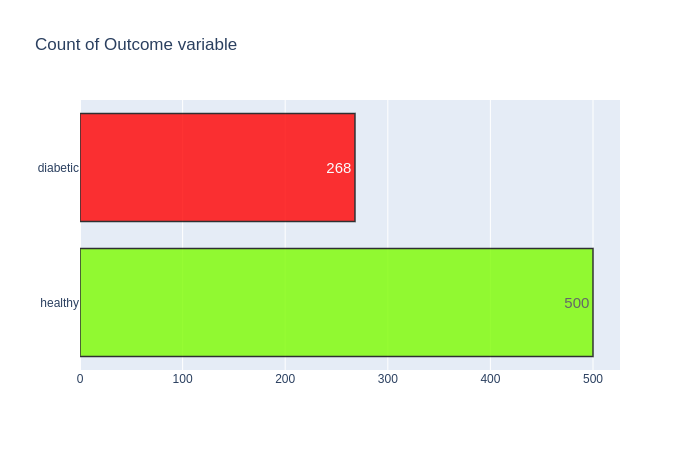
\includegraphics[width=1\textwidth]{1.png}
\caption{\label{fig:8} Diabetic v/s Healthy Subject Count.}
\end{figure}

\begin{figure}[ht]
\centering
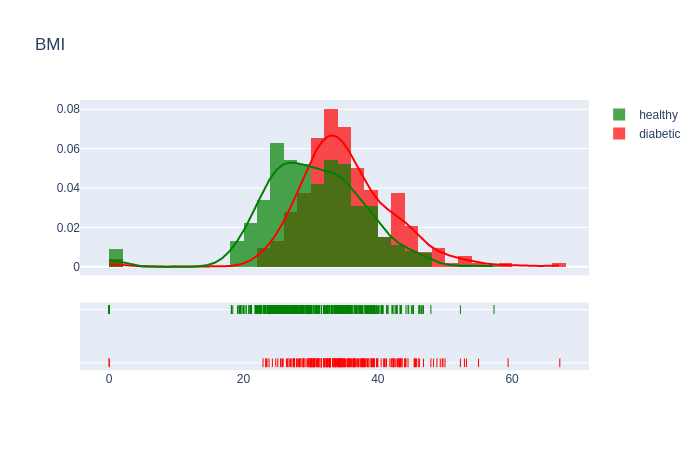
\includegraphics[width=1\textwidth]{10.png}
\caption{\label{fig:1} Subject distribution across Body Mass Index range.}
\end{figure}

\begin{figure}[ht]
\centering
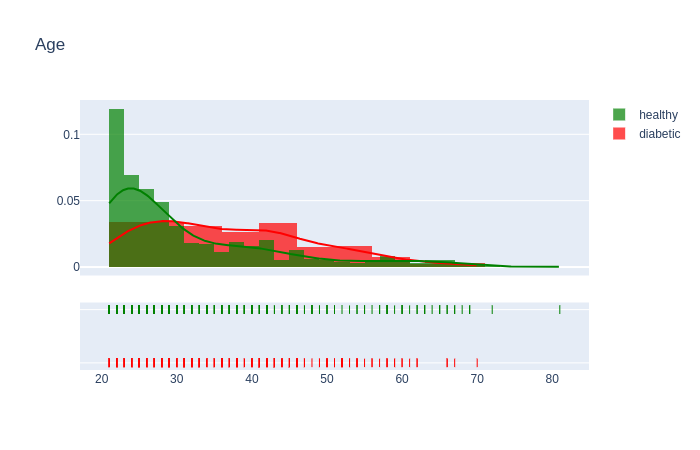
\includegraphics[width=1\textwidth]{11.png}
\caption{\label{fig:2} Subject distribution across age.}
\end{figure}

\begin{figure}[ht]
\centering
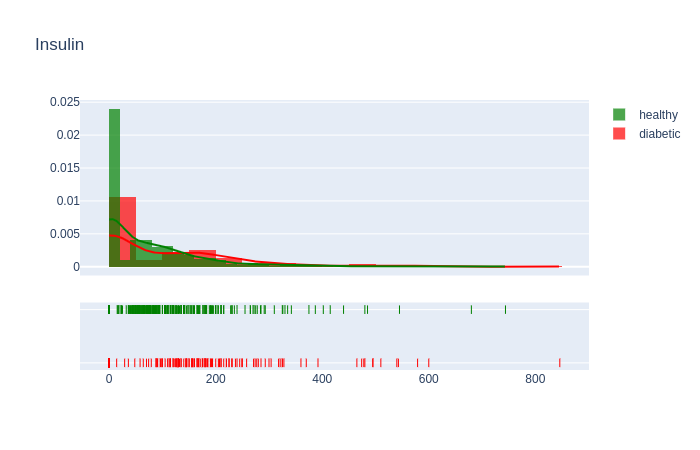
\includegraphics[width=1\textwidth]{14.png}
\caption{\label{fig:5} Subjects Insulin Distribution across ranges.}
\end{figure}

\begin{figure}[ht]
\centering
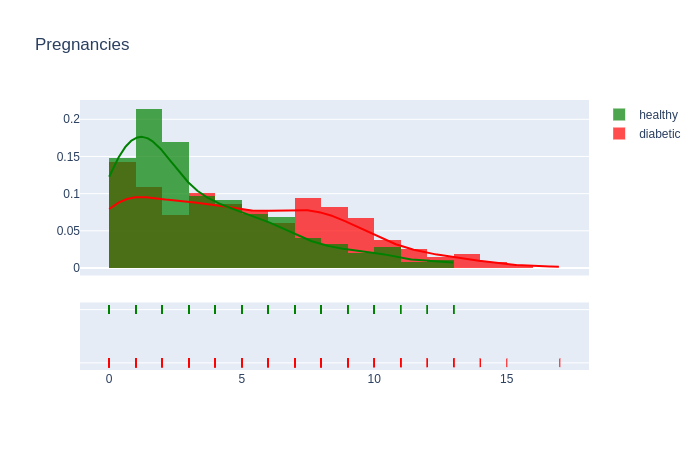
\includegraphics[width=1\textwidth]{12.png}
\caption{\label{fig:3} Subjects distribution via Pregnancies.}
\end{figure}

\begin{figure}[ht]
\centering
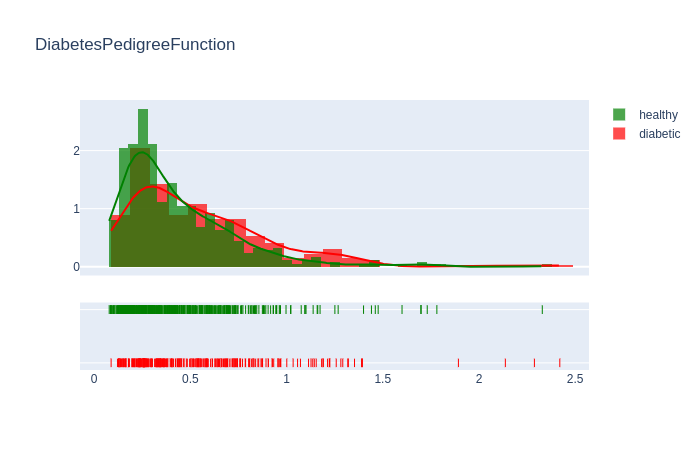
\includegraphics[width=1\textwidth]{13.png}
\caption{\label{fig:4} Subjects distribution via Diabetes Pedigree Function.}
\end{figure}


\begin{figure}[ht]
\centering
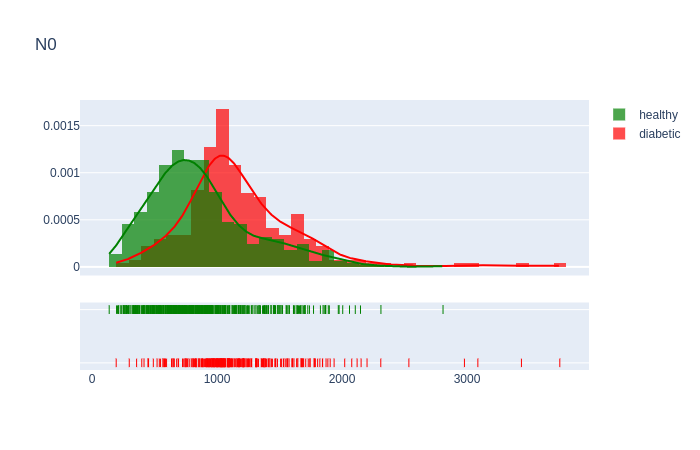
\includegraphics[width=1\textwidth]{15.png}
\caption{\label{fig:6} Plot of N0}
\end{figure}


\begin{figure}[ht]
\centering
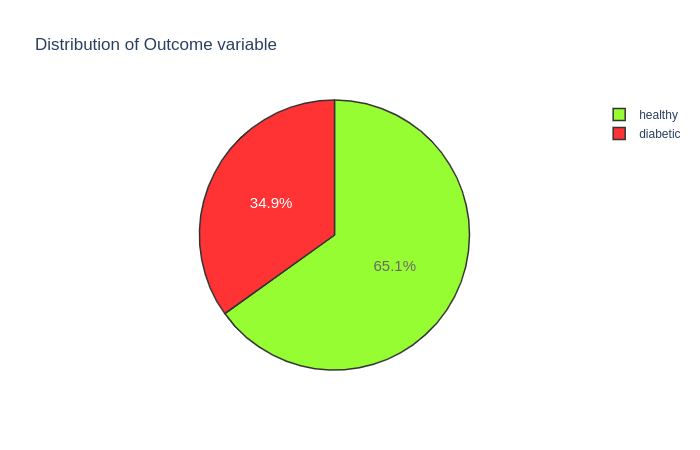
\includegraphics[width=1\textwidth]{2.png}
\caption{\label{fig:9} Diabetic v/s Healthy Subjects Percentage.}
\end{figure}

\begin{figure}[ht]
\centering
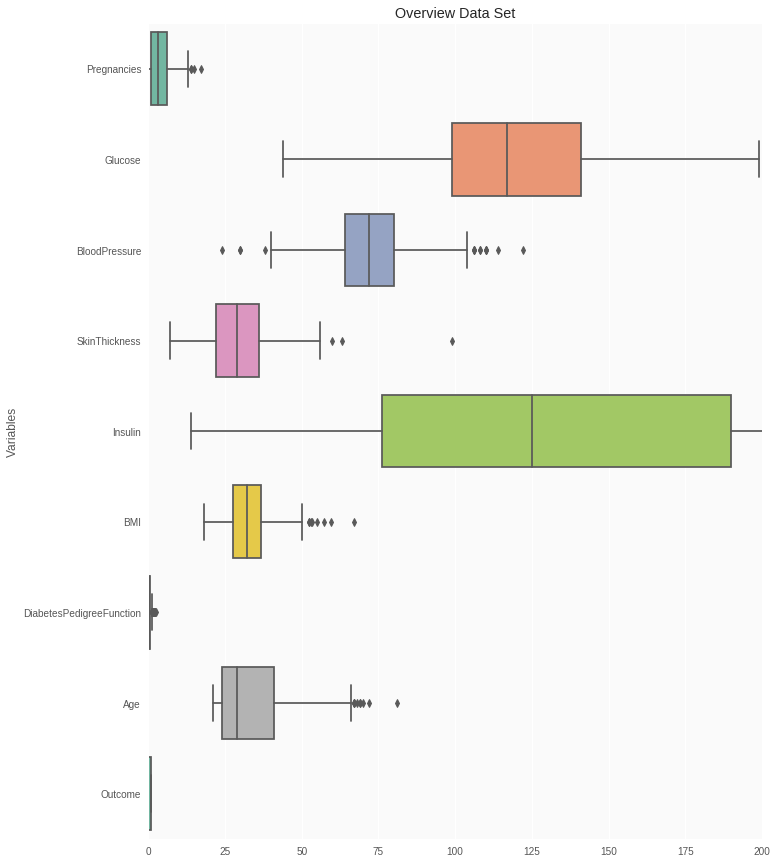
\includegraphics[width=1\textwidth]{3.png}
\caption{\label{fig:10} Boxplot for all attributes with outliers.}
\end{figure}

\begin{figure}[ht]
\centering
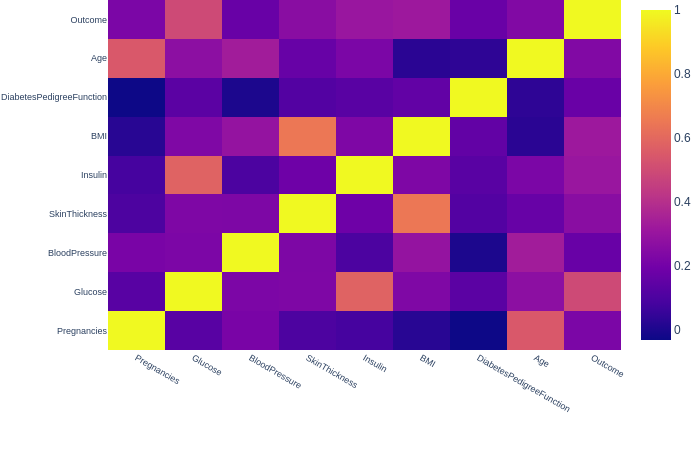
\includegraphics[width=1\textwidth]{4a.png}
\caption{\label{fig:11} Heatmap using Pearsons Correlation Coefficient.}
\end{figure}

\begin{figure}[ht]
\centering
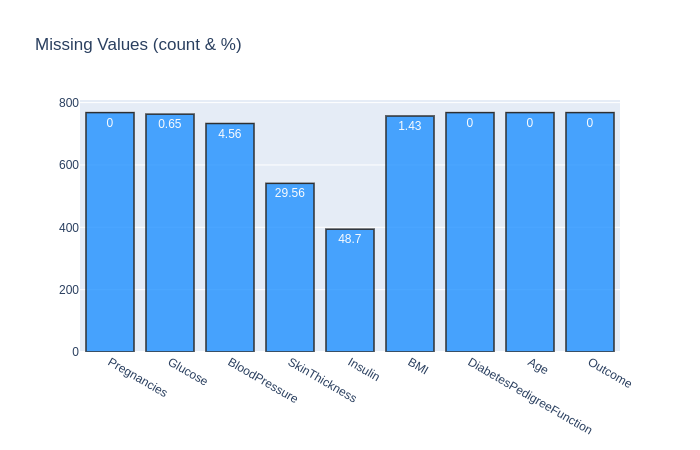
\includegraphics[width=1\textwidth]{4.png}
\caption{\label{fig:12} Number of missing values in count and percentage.}
\end{figure}

\begin{figure}[ht]
\centering
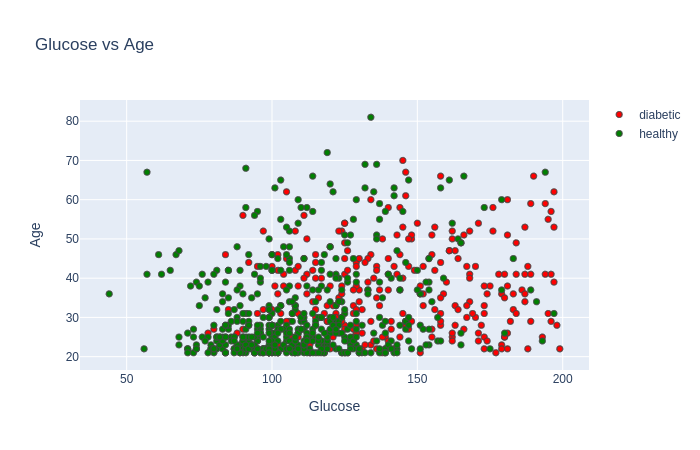
\includegraphics[width=1\textwidth]{5.png}
\caption{\label{fig:13} Glucose v/s Age scatterplot.}
\end{figure}


\begin{figure}[ht]
\centering
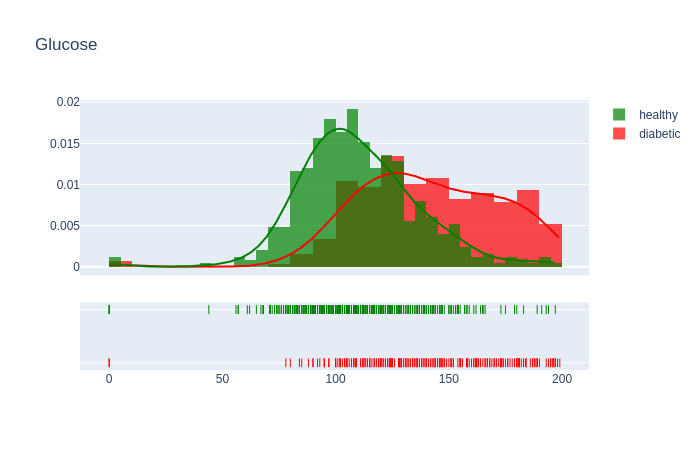
\includegraphics[width=1\textwidth]{7.png}
\caption{\label{fig:15} Subjects glucose distribution.}
\end{figure}

\begin{figure}[ht]
\centering
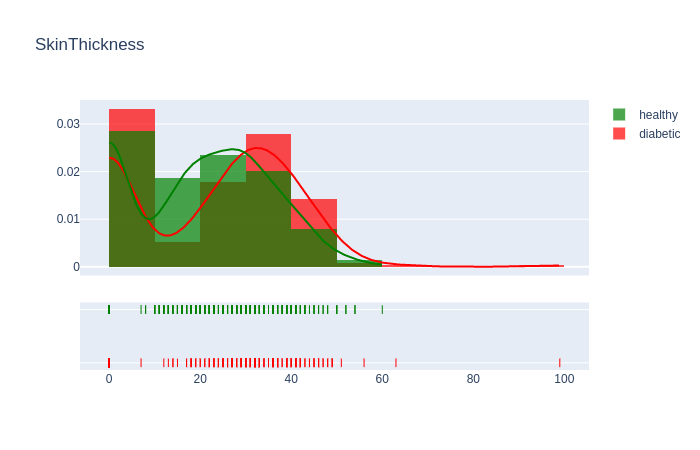
\includegraphics[width=1\textwidth]{8.png}
\caption{\label{fig:16} Skin Thickness distribution of subjects.}
\end{figure}

\begin{figure}[ht]
\centering
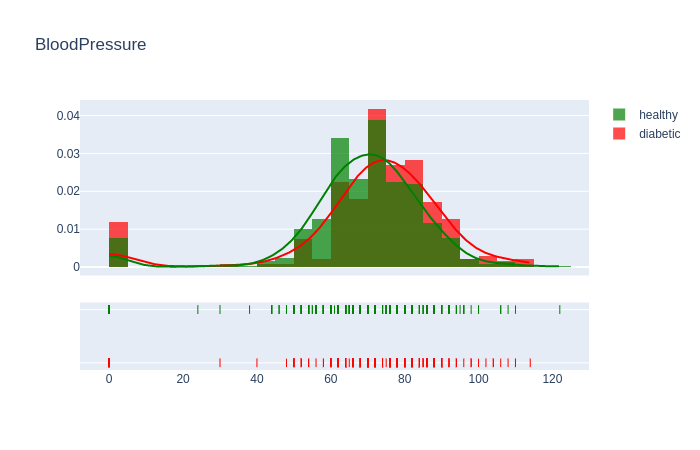
\includegraphics[width=1\textwidth]{9.png}
\caption{\label{fig:17} Blood Pressure distribution of subjects.}
\end{figure}

\begin{figure}[ht]
\centering
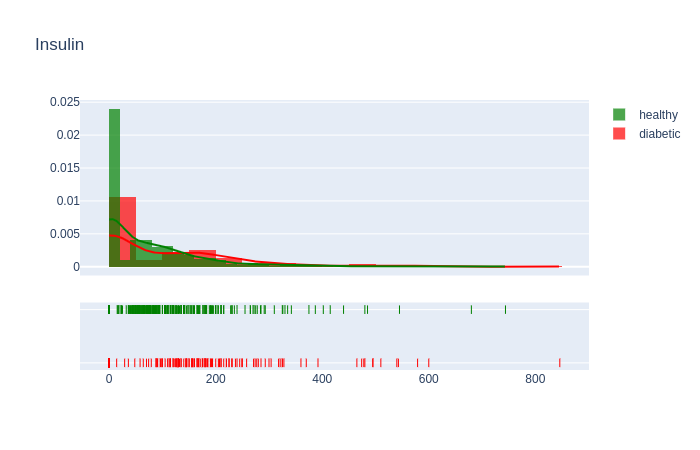
\includegraphics[width=1\textwidth]{6.png}
\caption{\label{fig:14} Subjects Insulin distributon.}
\end{figure}

\begin{figure}[ht]
\centering
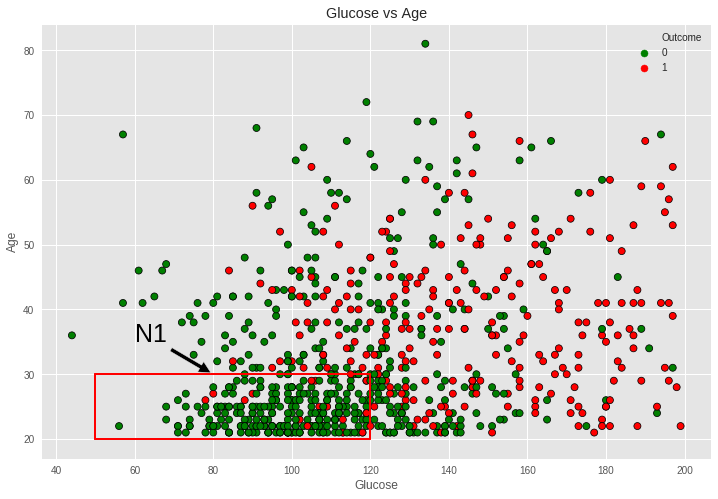
\includegraphics[width=1\textwidth]{download(1).png}
\caption{\label{fig:18} New feature N1.}
\end{figure}

\begin{figure}[ht]
\centering
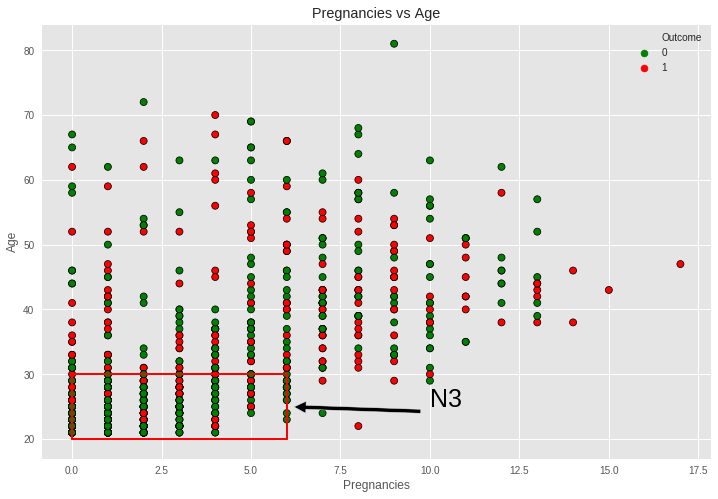
\includegraphics[width=1\textwidth]{download(2).png}
\caption{\label{fig:19} New feature N3.}
\end{figure}

\begin{figure}[ht]
\centering
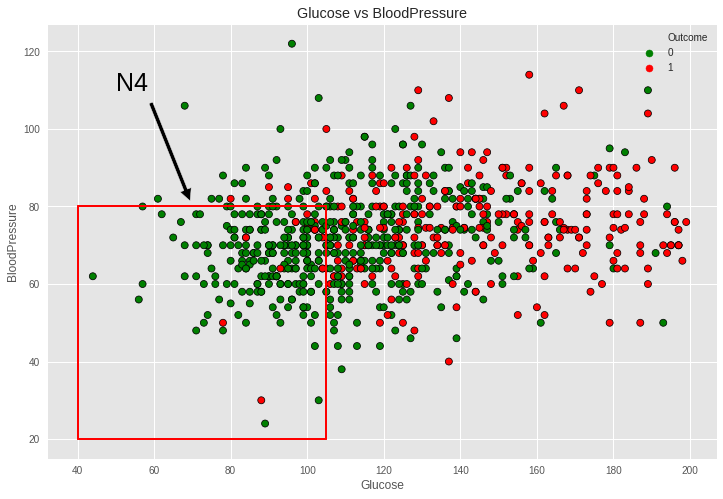
\includegraphics[width=1\textwidth]{download(3).png}
\caption{\label{fig:20}  New feature N4.}
\end{figure}

\begin{figure}[ht]
\centering
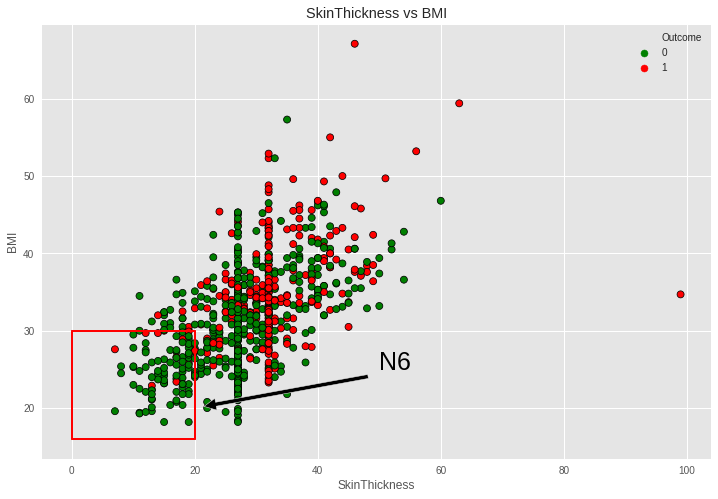
\includegraphics[width=1\textwidth]{download(4).png}
\caption{\label{fig:21}  New feature N6.}
\end{figure}

\begin{figure}[ht]
\centering
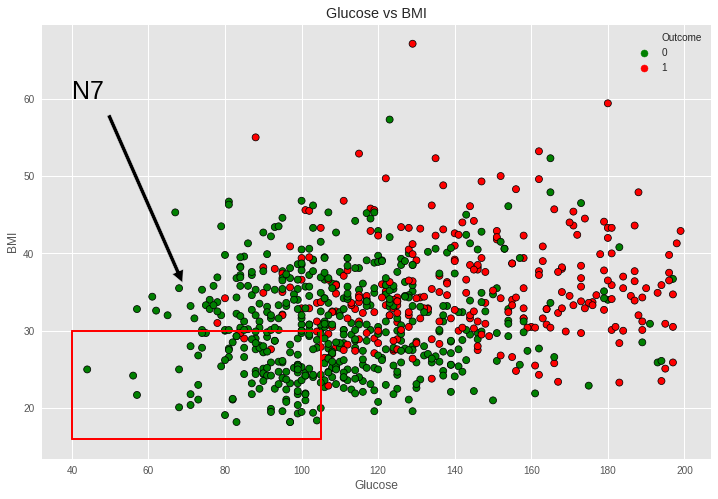
\includegraphics[width=1\textwidth]{download(5).png}
\caption{\label{fig:22}  New feature N7.}
\end{figure}

\begin{figure}[ht]
\centering
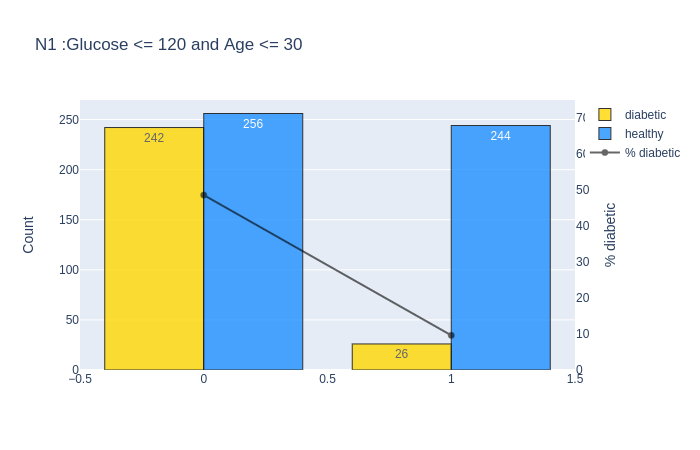
\includegraphics[width=1\textwidth]{newplot(13).png}
\caption{\label{fig:23} N1 barplot for diabetic and healthy population.}
\end{figure}

\begin{figure}[ht]
\centering
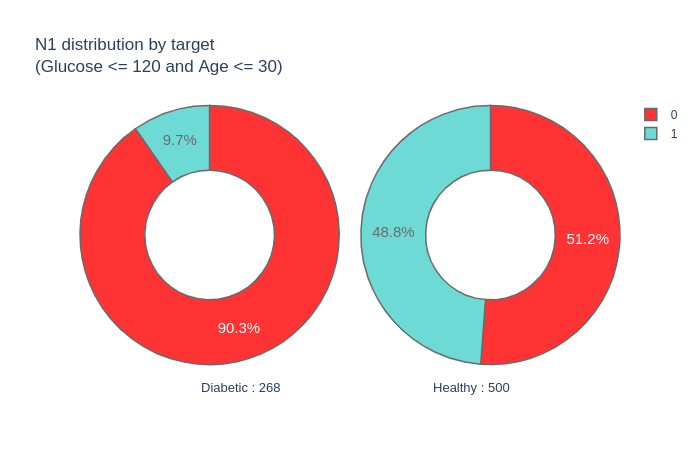
\includegraphics[width=1\textwidth]{newplot(14).png}
\caption{\label{fig:24} N1 distribution in percentage.}
\end{figure}

\begin{figure}[ht]
\centering
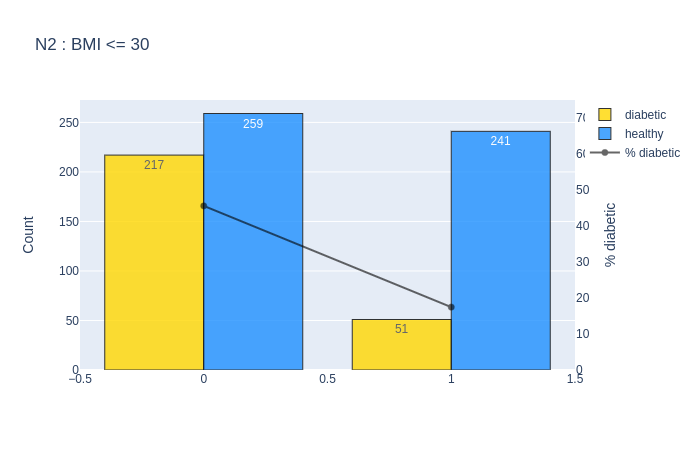
\includegraphics[width=1\textwidth]{newplot(15).png}
\caption{\label{fig:25} N2 barplot for diabetic and healthy population.}
\end{figure}

\begin{figure}[ht]
\centering
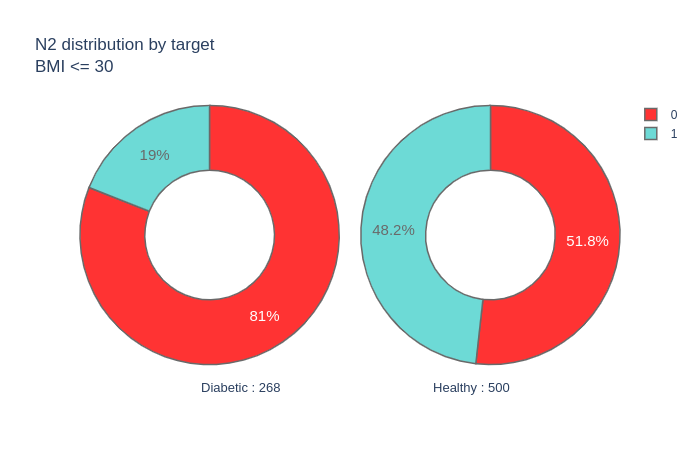
\includegraphics[width=1\textwidth]{newplot(16).png}
\caption{\label{fig:26} N2 distribution in percentage.}
\end{figure}

\begin{figure}[ht]
\centering
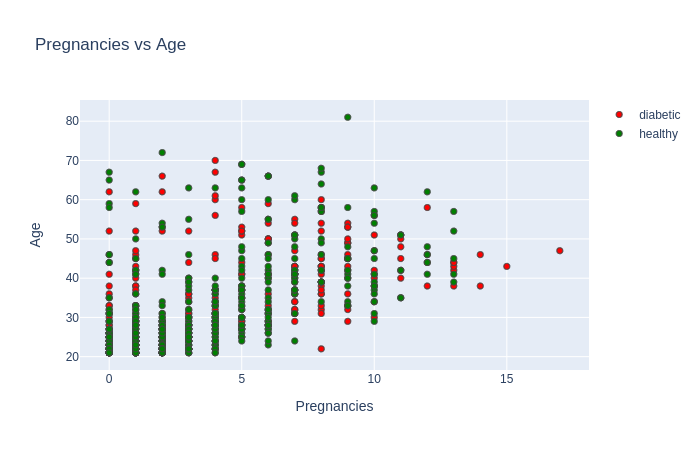
\includegraphics[width=1\textwidth]{newplot(17).png}
\caption{\label{fig:27} Pregnancies v/s age scatterplot.}
\end{figure}

\begin{figure}[ht]
\centering
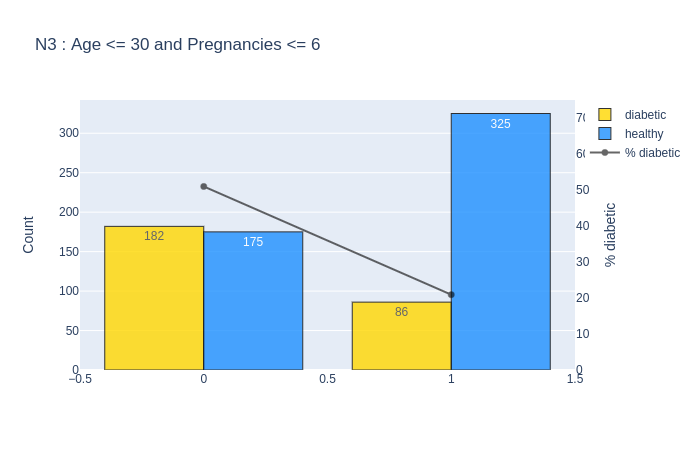
\includegraphics[width=1\textwidth]{newplot(18).png}
\caption{\label{fig:28} N3 barplot for diabetic and healthy population.}
\end{figure}

\begin{figure}[ht]
\centering
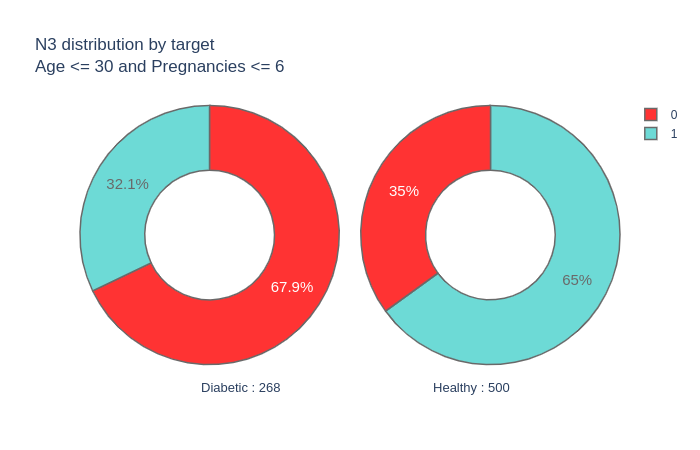
\includegraphics[width=1\textwidth]{newplot(19).png}
\caption{\label{fig:29} N3 distribution in percentage.}
\end{figure}

\begin{figure}[ht]
\centering
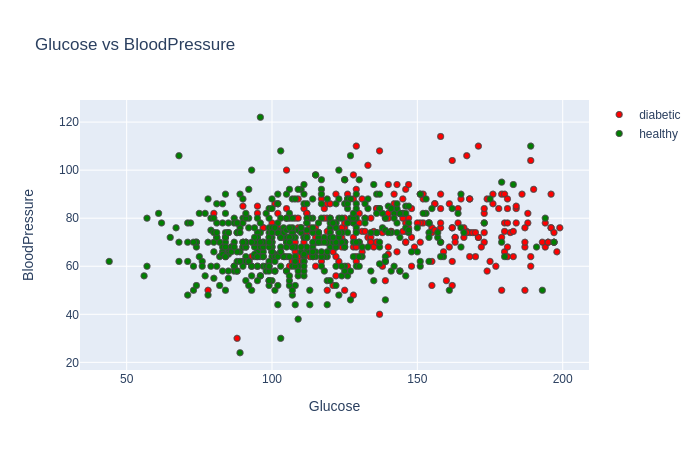
\includegraphics[width=1\textwidth]{newplot(20).png}
\caption{\label{fig:30} Glucose v/s Blood Pressure scatterplot.}
\end{figure}

\begin{figure}[ht]
\centering
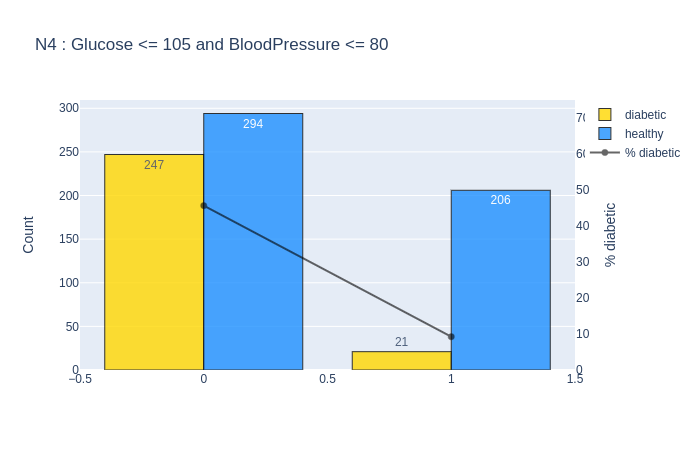
\includegraphics[width=1\textwidth]{newplot(21).png}
\caption{\label{fig:31} N4 barplot for diabetic and healthy population.}
\end{figure}

\begin{figure}[ht]
\centering
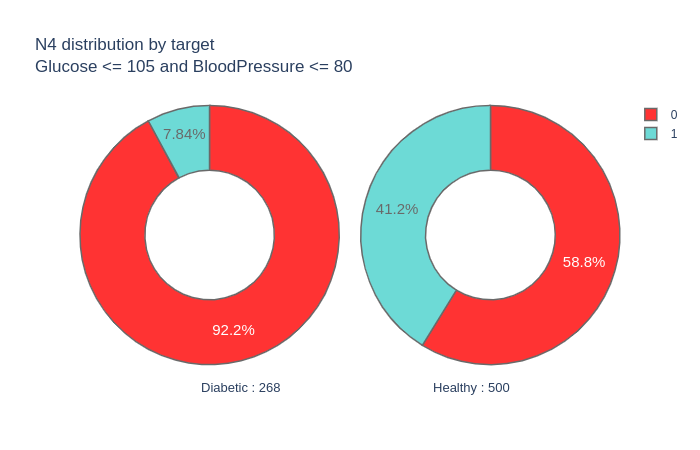
\includegraphics[width=1\textwidth]{newplot(22).png}
\caption{\label{fig:32} N4 distribution by target.}
\end{figure}

\begin{figure}[ht]
\centering
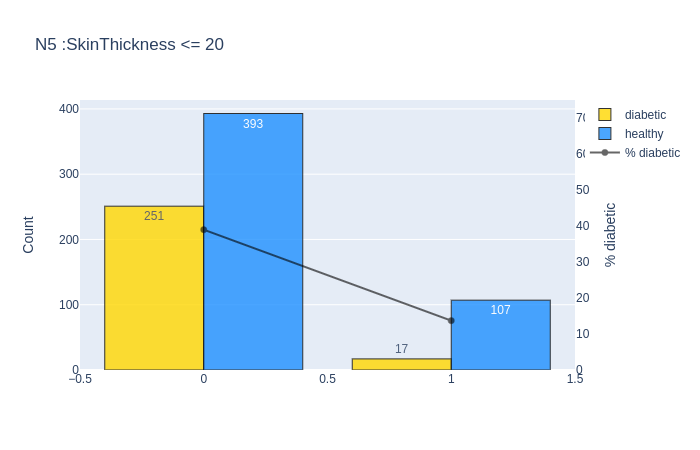
\includegraphics[width=1\textwidth]{newplot(23).png}
\caption{\label{fig:33} N5 barplot for diabetic and healthy population.}
\end{figure}

\begin{figure}[ht]
\centering
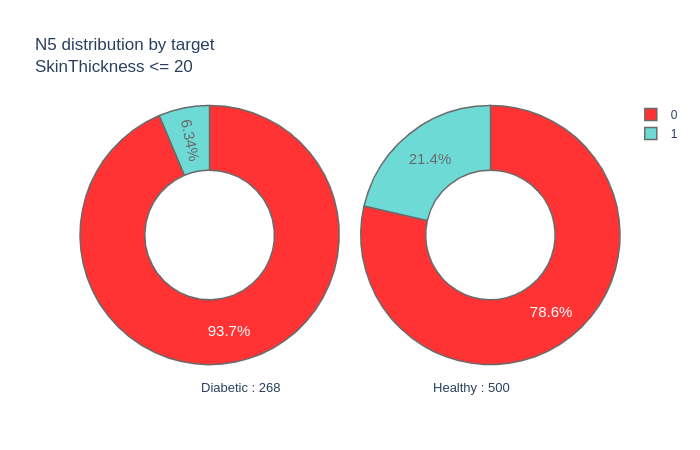
\includegraphics[width=1\textwidth]{newplot(24).png}
\caption{\label{fig:34} N5 distribution by target.}
\end{figure}

\begin{figure}[ht]
\centering
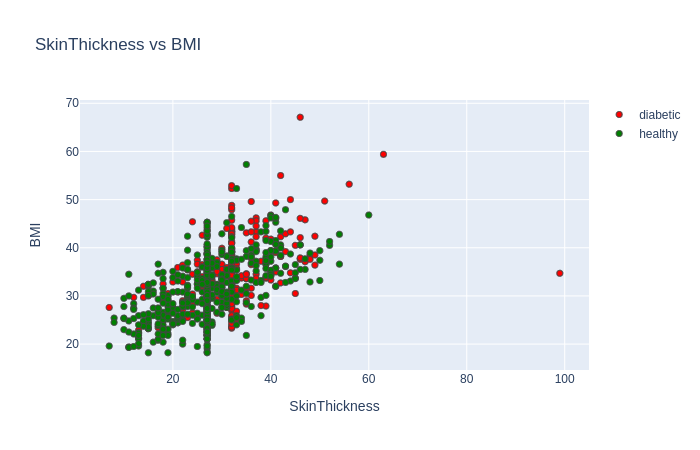
\includegraphics[width=1\textwidth]{newplot(25).png}
\caption{\label{fig:35} Skin Thickness v/s BMI scatterplot.}
\end{figure}

\begin{figure}[ht]
\centering
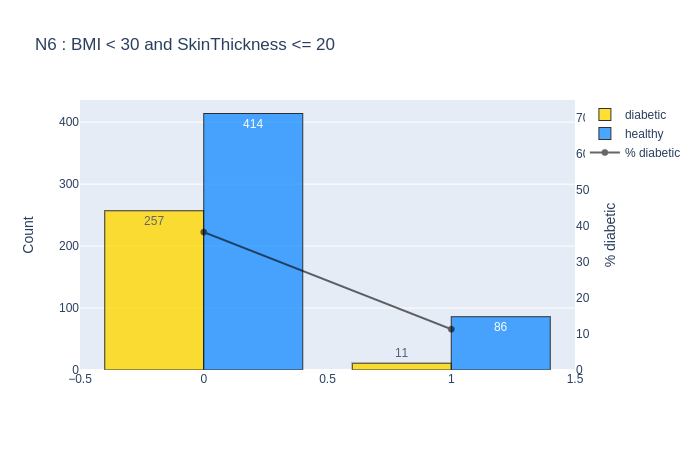
\includegraphics[width=1\textwidth]{newplot(26).png}
\caption{\label{fig:36} N6 barplot for diabetic and healthy population.}
\end{figure}

\begin{figure}[ht]
\centering
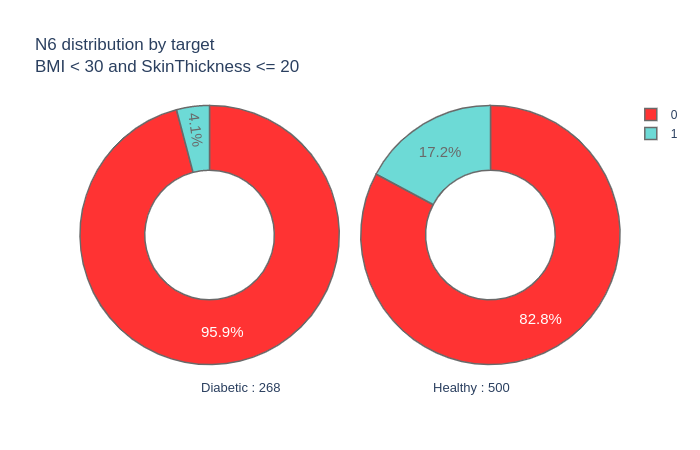
\includegraphics[width=1\textwidth]{newplot(27).png}
\caption{\label{fig:37} N6 distribution by target.}
\end{figure}

\begin{figure}[ht]
\centering
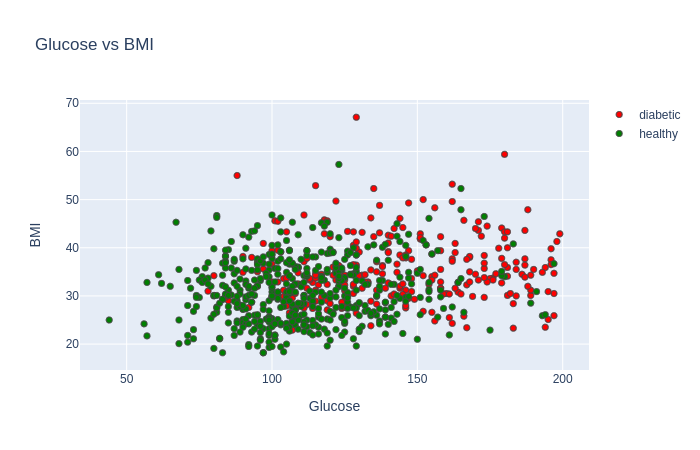
\includegraphics[width=1\textwidth]{newplot(28).png}
\caption{\label{fig:38} Glucose v/s Body Mass Index scatterplot.}
\end{figure}

\begin{figure}[ht]
\centering
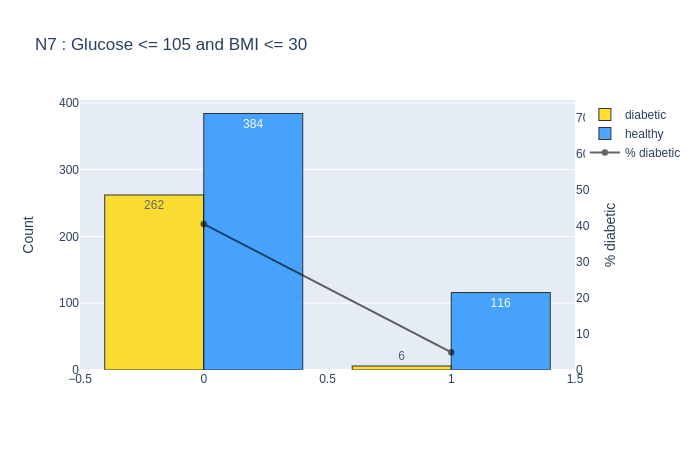
\includegraphics[width=1\textwidth]{newplot(29).png}
\caption{\label{fig:39} N7 barplot for diabetic and healthy population.}
\end{figure}

\begin{figure}[ht]
\centering
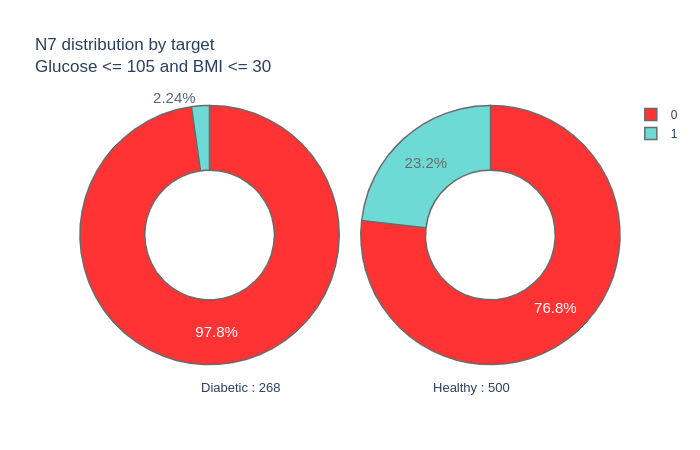
\includegraphics[width=1\textwidth]{newplot(30).png}
\caption{\label{fig:40} N7 distribution by target.}
\end{figure}

\begin{figure}[ht]
\centering
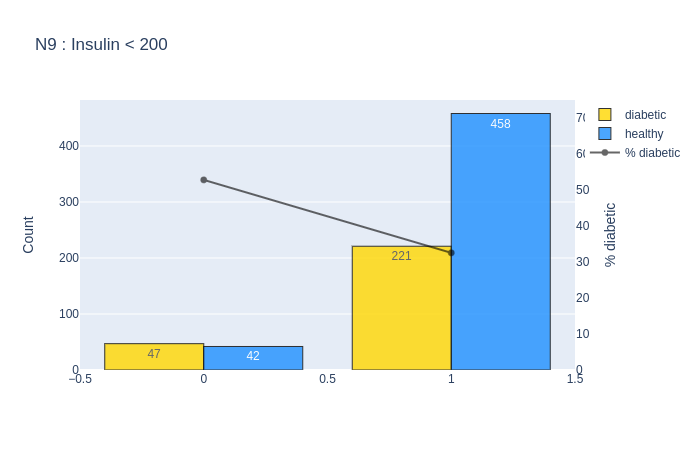
\includegraphics[width=1\textwidth]{newplot(32).png}
\caption{\label{fig:41} N9 barplot for diabetic and healthy population.}
\end{figure}

\begin{figure}[ht]
\centering
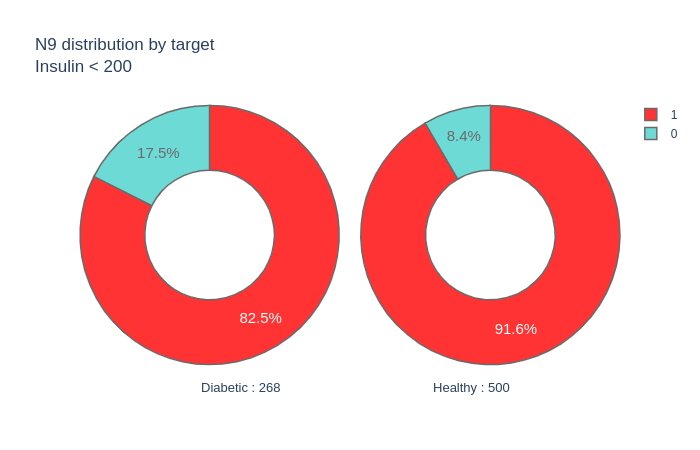
\includegraphics[width=1\textwidth]{newplot(33).png}
\caption{\label{fig:42} N9 distribution by target.}
\end{figure}

\begin{figure}[ht]
\centering
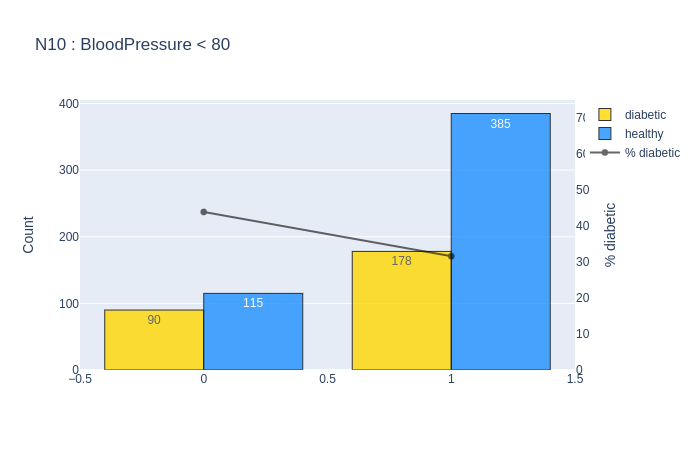
\includegraphics[width=1\textwidth]{newplot(34).png}
\caption{\label{fig:43} N10 barplot for diabetic and healthy population.}
\end{figure}

\begin{figure}[ht]
\centering
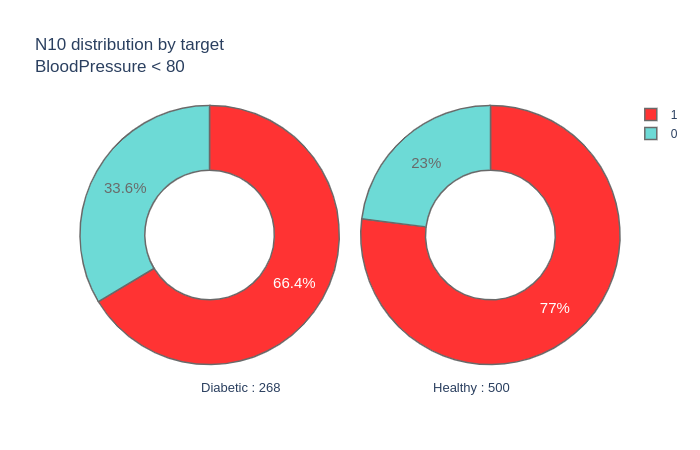
\includegraphics[width=1\textwidth]{newplot(35).png}
\caption{\label{fig:44} N10 distribution by target.}
\end{figure}

\begin{figure}[ht]
\centering
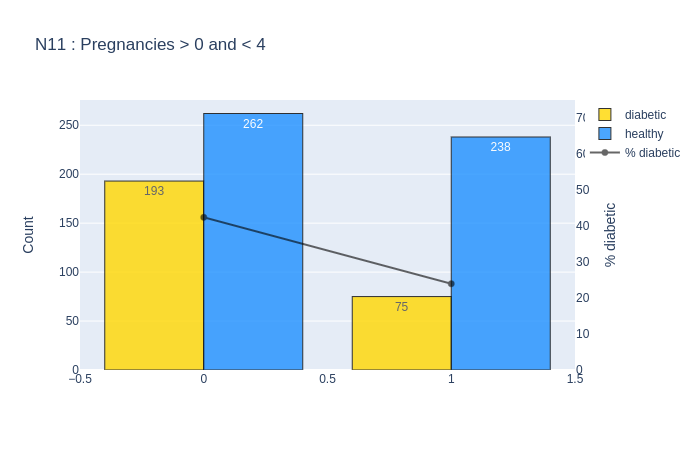
\includegraphics[width=1\textwidth]{newplot(37).png}
\caption{\label{fig:45} N11 barplot for diabetic and healthy population.}
\end{figure}

\begin{figure}[ht]
\centering
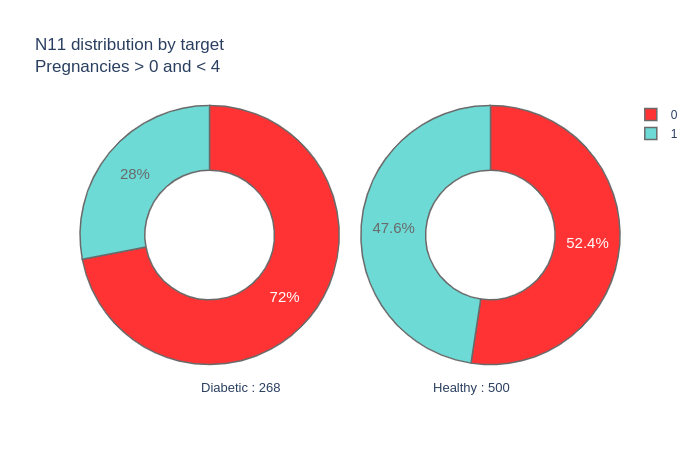
\includegraphics[width=1\textwidth]{newplot(38).png}
\caption{\label{fig:46} N11 distribution by target.}
\end{figure}

\begin{figure}[ht]
\centering
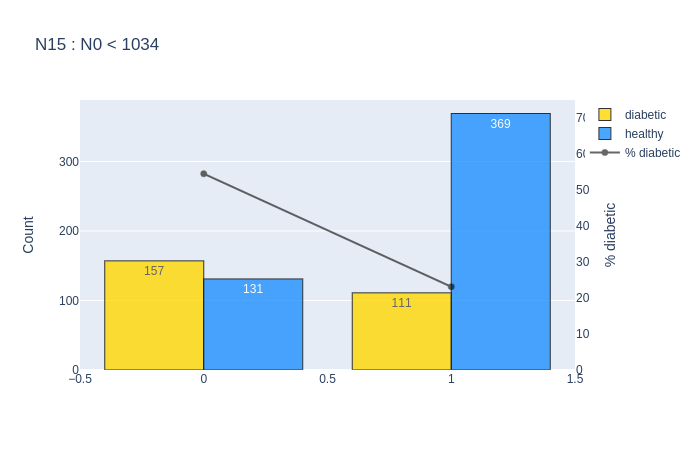
\includegraphics[width=1\textwidth]{newplot(40).png}
\caption{\label{fig:47} N15 barplot for diabetic and healthy population.}
\end{figure}

\begin{figure}[ht]
\centering
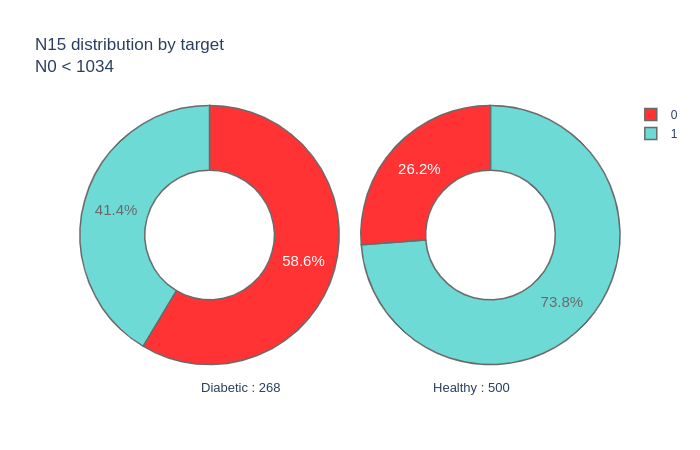
\includegraphics[width=1\textwidth]{newplot(41).png}
\caption{\label{fig:48} N15 distribution by target.}
\end{figure}

\begin{figure}[ht]
\centering
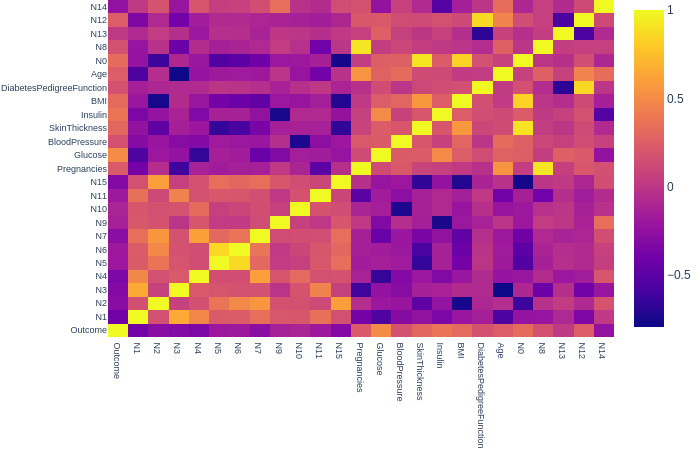
\includegraphics[width=1\textwidth]{newplot(42).png}
\caption{\label{fig:49} Extended heatmap with new features combined.}
\end{figure}

\clearpage
\newpage
\section{Conclusion}

\newpage

\nocite{*}
\bibliography{bib} 
\bibliographystyle{plain}

\end{document}
